\documentclass{report}
\usepackage[italian]{babel}
\usepackage[utf8]{inputenc}
\usepackage{titlesec}
\usepackage[export]{adjustbox}
\usepackage{hyperref}
\usepackage{geometry}

\usepackage{caption}
\usepackage{amsmath}
\usepackage{natbib}

\captionsetup[table]{position=bottom}

%\usepackage[cm]{fullpage}

% some very useful LaTeX packages include:

%\usepackage{cite}      % Written by Donald Arseneau
                        % V1.6 and later of IEEEtran pre-defines the format
                        % of the cite.sty package \cite{} output to follow
                        % that of IEEE. Loading the cite package will
                        % result in citation numbers being automatically
                        % sorted and properly "ranged". i.e.,
                        % [1], [9], [2], [7], [5], [6]
                        % (without using cite.sty)
                        % will become:
                        % [1], [2], [5]--[7], [9] (using cite.sty)
                        % cite.sty's \cite will automatically add leading
                        % space, if needed. Use cite.sty's noadjust option
                        % (cite.sty V3.8 and later) if you want to turn this
                        % off. cite.sty is already installed on most LaTeX
                        % systems. The latest version can be obtained at:
                        % http://www.ctan.org/tex-archive/macros/latex/contrib/supported/cite/
\usepackage[inline]{enumitem}

\usepackage{graphicx}   % Written by David Carlisle and Sebastian Rahtz
                        % Required if you want graphics, photos, etc.
                        % graphicx.sty is already installed on most LaTeX
                        % systems. The latest version and documentation can
                        % be obtained at:
                        % http://www.ctan.org/tex-archive/macros/latex/required/graphics/
                        % Another good source of documentation is "Using
                        % Imported Graphics in LaTeX2e" by Keith Reckdahl
                        % which can be found as esplatex.ps and epslatex.pdf
                        % at: http://www.ctan.org/tex-archive/info/

%\usepackage{psfrag}    % Written by Craig Barratt, Michael C. Grant,
                        % and David Carlisle
                        % This package allows you to substitute LaTeX
                        % commands for text in imported EPS graphic files.
                        % In this way, LaTeX symbols can be placed into
                        % graphics that have been generated by other
                        % applications. You must use latex->dvips->ps2pdf
                        % workflow (not direct pdf output from pdflatex) if
                        % you wish to use this capability because it works
                        % via some PostScript tricks. Alternatively, the
                        % graphics could be processed as separate files via
                        % psfrag and dvips, then converted to PDF for
                        % inclusion in the main file which uses pdflatex.
                        % Docs are in "The PSfrag System" by Michael C. Grant
                        % and David Carlisle. There is also some information
                        % about using psfrag in "Using Imported Graphics in
                        % LaTeX2e" by Keith Reckdahl which documents the
                        % graphicx package (see above). The psfrag package
                        % and documentation can be obtained at:
                        % http://www.ctan.org/tex-archive/macros/latex/contrib/supported/psfrag/

%\usepackage{subfigure} % Written by Steven Douglas Cochran
                        % This package makes it easy to put subfigures
                        % in your figures. i.e., "figure 1a and 1b"
                        % Docs are in "Using Imported Graphics in LaTeX2e"
                        % by Keith Reckdahl which also documents the graphicx
                        % package (see above). subfigure.sty is already
                        % installed on most LaTeX systems. The latest version
                        % and documentation can be obtained at:
                        % http://www.ctan.org/tex-archive/macros/latex/contrib/supported/subfigure/

\usepackage{url}        % Written by Donald Arseneau
                        % Provides better support for handling and breaking
                        % URLs. url.sty is already installed on most LaTeX
                        % systems. The latest version can be obtained at:
                        % http://www.ctan.org/tex-archive/macros/latex/contrib/other/misc/
                        % Read the url.sty source comments for usage information.

%\usepackage{stfloats}  % Written by Sigitas Tolusis
                        % Gives LaTeX2e the ability to do double column
                        % floats at the bottom of the page as well as the top.
                        % (e.g., "\begin{figure*}[!b]" is not normally
                        % possible in LaTeX2e). This is an invasive package
                        % which rewrites many portions of the LaTeX2e output
                        % routines. It may not work with other packages that
                        % modify the LaTeX2e output routine and/or with other
                        % versions of LaTeX. The latest version and
                        % documentation can be obtained at:
                        % http://www.ctan.org/tex-archive/macros/latex/contrib/supported/sttools/
                        % Documentation is contained in the stfloats.sty
                        % comments as well as in the presfull.pdf file.
                        % Do not use the stfloats baselinefloat ability as
                        % IEEE does not allow \baselineskip to stretch.
                        % Authors submitting work to the IEEE should note
                        % that IEEE rarely uses double column equations and
                        % that authors should try to avoid such use.
                        % Do not be tempted to use the cuted.sty or
                        % midfloat.sty package (by the same author) as IEEE
                        % does not format its papers in such ways.
\usepackage{amssymb}
\usepackage{amsmath}    % From the American Mathematical Society
                        % A popular package that provides many helpful commands
                        % for dealing with mathematics. Note that the AMSmath
                        % package sets \interdisplaylinepenalty to 10000 thus
                        % preventing page breaks from occurring within multiline
                        % equations. Use:
%\interdisplaylinepenalty=2500
                        % after loading amsmath to restore such page breaks
                        % as IEEEtran.cls normally does. amsmath.sty is already
                        % installed on most LaTeX systems. The latest version
                        % and documentation can be obtained at:
                        % http://www.ctan.org/tex-archive/macros/latex/required/amslatex/math/
\usepackage{latexsym}
\usepackage{amsthm}
\usepackage{blindtext}
\usepackage{calligra}
\usepackage{fancyhdr}
\usepackage{amsmath}
\usepackage{amssymb}
\usepackage{listings}
\usepackage[usenames]{color}
\newcommand{\fncyblank}{\fancyhf{}}
\usepackage{verbatim}
\usepackage[htt]{hyphenat}
\graphicspath{{./res/}}

%\setcounter{secnumdepth}{4}

\setlength{\parindent}{0pt}
\setlength{\parskip}{0.3em}

\usepackage{algorithm}
\usepackage{algpseudocode}
\algrenewcommand{\algorithmiccomment}[1]{$\left(\text{#1}\right)$}
\usepackage{color}

\definecolor{ideanumber}{rgb}{0.0,0.0,1.0}
\definecolor{ideacomment}{rgb}{0.5,0.5,0.5}
\definecolor{ideakeyword}{rgb}{0.0,0.0,0.5}
\definecolor{ideastring}{rgb}{0.0,0.5,0.0}

\PassOptionsToPackage{hyphens}{url}

\usepackage{listings}
\lstset{frame=tb,
    language=Java,
    aboveskip=3mm,
    belowskip=3mm,
    showstringspaces=false,
    columns=flexible,
    basicstyle={\small\ttfamily},
    numbers=left,
    numbersep=2pt,                   % how far the line-numbers are from the code
    numberstyle=\tiny\color{ideacomment},
    keywordstyle=\color{ideakeyword},
    commentstyle=\color{ideacomment},
    stringstyle=\color{ideastring},
    breaklines=true,
    breakatwhitespace=true,
    tabsize=4
}

% Other popular packages for formatting tables and equations include:

%\usepackage{array}
% Frank Mittelbach's and David Carlisle's array.sty which improves the
% LaTeX2e array and tabular environments to provide better appearances and
% additional user controls. array.sty is already installed on most systems.
% The latest version and documentation can be obtained at:
% http://www.ctan.org/tex-archive/macros/latex/required/tools/

% V1.6 of IEEEtran contains the IEEEeqnarray family of commands that can
% be used to generate multiline equations as well as matrices, tables, etc.

% Also of notable interest:
% Scott Pakin's eqparbox package for creating (automatically sized) equal
% width boxes. Available:
% http://www.ctan.org/tex-archive/macros/latex/contrib/supported/eqparbox/

% *** Do not adjust lengths that control margins, column widths, etc. ***
% *** Do not use packages that alter fonts (such as pslatex).         ***
% There should be no need to do such things with IEEEtran.cls V1.6 and later.
\newcommand\textsup[1]{$^{\text{#1}}$}
\newcommand\textsub[1]{$_{\text{#1}}$}



% To use paragraph like a subsubsubsection
\setcounter{secnumdepth}{4}
\titleformat{\paragraph}
{\normalfont\normalsize\bfseries}{\theparagraph}{1em}{}
\titlespacing*{\paragraph}
{0pt}{3.25ex plus 1ex minus .2ex}{1.5ex plus .2ex}

\hypersetup{
    bookmarks=true,         % show bookmarks bar?
    unicode=false,          % non-Latin characters in Acrobat’s bookmarks
    pdftoolbar=true,        % show Acrobat’s toolbar?
    pdfmenubar=true,        % show Acrobat’s menu?
    pdffitwindow=false,     % window fit to page when opened
    pdfstartview={FitH},    % fits the width of the page to the window
    pdftitle={My title},    % title
    pdfauthor={Author},     % author
    pdfsubject={Subject},   % subject of the document
    pdfcreator={Creator},   % creator of the document
    pdfproducer={Producer}, % producer of the document
    pdfkeywords={keyword1, key2, key3}, % list of keywords
    pdfnewwindow=true,      % links in new PDF window
    colorlinks=true,       % false: boxed links; true: colored links
    linkcolor=black,          % color of internal links (change box color with linkbordercolor)
    citecolor=black,        % color of links to bibliography
    filecolor=black,      % color of file links
    urlcolor=blue           % color of external links
}

\begin{document}

\begin{titlepage}
	\centering
	{\scshape\LARGE Università di Bologna \par}
	\vspace{1cm}
	{\scshape\Large Elaborato di progetto per l'esame di Paradigmi di Programmazione e Sviluppo\par}
	\vspace{1.5cm}
	{\Huge\bfseries Distributed Chat Service\par}
	\vspace{2cm}
	{\Large     
	Nicola Piscaglia\\
    \texttt{nicola.piscaglia2@studio.unibo.it}\\
    \vspace{0.5cm}
    Mattia Vandi\\
    \texttt{mattia.vandi@studio.unibo.it}\\
    \vspace{0.5cm}
    Alessandro Gnucci\\
    \texttt{alessandro.gnucci@studio.unibo.it}\\
    \vspace{0.5cm}
    Martina Magnani\\
    \texttt{martina.magnani8@studio.unibo.it}\par}
	\vfill
	\vfill

% Bottom of the page
	{\large A.A. 2017/2018 \par}
\end{titlepage}

\tableofcontents

\listoffigures

\listoftables

\chapter{Processo di Sviluppo}
\section{Metodologia di sviluppo}
Relativamente al processo di sviluppo è stato deciso di adottare e testare una
metodologia \textbf{Agile Scrum-like}. \newline
Nella versione da noi utilizzata
i membri del team sono allo stesso livello, non esiste infatti
uno \textit{Scrum Leader}, ne uno \textit{Scrum Manager}. Il ruolo del \textit{Product Manager} è
stato ricoperto da \textit{Nicola Piscaglia}. 
Come alternativa ad una vera e propria \textit{Kanban} abbiamo
deciso di usare \textbf{Trello}: qui, come fasi dello sprint abbiamo usato \textit{"Backlog"}, \textit{"ToDo"}, \textit{"Design"}, 
\textit{"Develop"}, \textit{"Review"} e \textit{"Done"}. Abbiamo reputato corretto fare
sprints con cadenza settimanale, poichè così è possibile ottenere una buona quantità di feedback
dall'utente e numerose opportunità per imparare e migliorare. \newline
All'inizio del processo di sviluppo abbiamo delineato il \textit{Product Backlog}, contenente gli items, 
con relativa priorità e dimensione stimata; inoltre, è stato fatto un primo sforzo per la modellazione del sistema
in termini di servizi e patterns architetturali, producendo: un diagramma relativo alla gerarchia dei servizi,
uno schema relazionale ed uno logico dei databases.
\newline
All' inizio di ogni settimana abbiamo fatto un meeting, tutti assieme,
per decidere quali elementi del \textit{Product Backlog} assegnare al
prossimo sprint, strutturando lo
\textit{Sprint Backlog}, delineando con più precisione la dimensione degli items. 
\\A seguito di ciò,
i membri del team hanno scelto gli items seguendo le priorità già delineate 
ed hanno iniziato a fare il design ed implementarne le features descritte tramite \textit{TDD}, senza più cambiare le decisioni
 relative agli items prese all'inizio dello sprint. 
 \\\textit{Il Test Driven Development} è un modello di sviluppo che prevede che la stesura dei tests sia fatta prima dell'implementazione e che lo sviluppo sia orientato esclusivamente all'obiettivo di passare i tests precedentemente predisposti. Più in dettaglio, \textit{TDD} prevede un breve ciclo di sviluppo in tre fasi: nella prima si scrive un test per la nuova funzione da sviluppare, nella seconda si sviluppa il codice necessario per passare il test; infine, nella terza si esegue il refactoring del codice per adeguarlo ad determinati standards di qualità.
\newline
Durante lo sviluppo, ogni singolo elemento del team ha la possibilità di fare \textit{Pull Requests} al 
\textit{Repo verità} (non si può fare push): a quel punto,
un altra persona del team controllerà la qualità del codice della singola \textit{PR} e, 
se tutto risulta a norma, farà merge nel branch dello sprint corrente.
Lo strumento di \textit{continuous integration} è stato configurato per permettere il merge di una pull request solo in caso di procedura di build andata a buon fine e solo se tutti i tests terminano con successo; Infine, è stato impostato lo stesso strumento in modo da
generare in automatico l'eseguibile del progetto.
\newline
Al termine di ogni \textit{Sprint} i componenti del team hanno preso parte ad un meeting, in cui sono state
poste in atto le fasi di \textit{Sprint Review} (per valutare il risultato dello Sprint e stabilire le priorit`a delle
prossime feature da portare a termine) e di \textit{Retrospective} (per analizzare il processo di sviluppo
allo scopo di migliorare la produttività del team).
\\
Si è reso necessario, a volte, contattare elementi del team tramite Skype o strumenti simili, 
senza riunire però tutti gli elementi, per risolvere problemi o per procedere con lo sviluppo.
Infine, gli items non completati entro la fine dello sprint sono stati semplicemente riportati
nello sprint successivo.

\section{Strumenti adottati}
I principali strumenti utilizzati durante l'intero processo di sviluppo sono i seguenti:
\begin{itemize}
\item \textbf{Git}: come sistema di versioning abbiamo optato per Git per la sua diffusione, velocità e semplicità di utilizzo;
\item \textbf{GitHub}: è stato scelto GitHub come servizio di hosting;
per il version control e per il repository, poichè permette ampia possibilità di integrazione con altri strumenti di sviluppo. Il repository è disponibile al seguente \href{https://github.com/GMPVTeam/pps17-distributed-chat-service}{link};
\item \textbf{GitFlow}: come metodologia di \textit{branching} all’interno del repository abbiamo adottato
GitFlow, poichè rende lo sviluppo parallelo molto semplice;
\item \textbf{Google Sheets}: la creazione e gestione del \textit{Product Backlog}, \textit{Sprint Backlog}, \textit{Sprint Review} e \textit{Sprint Retrospective} sono state fatte tramite Google Sheets, vista la sua semplicità di utilizzo. È possibile visualizzare i documenti predetti al seguente \href{https://docs.google.com/spreadsheets/d/13H6Xl3ZzywzSpik3gxQbl6CnDtzObbCIdqROZq82Zk4/edit?usp=sharing}{link};
\item \textbf{Gradle}: per la gestione della build di progetto è stato scelto Gradle, per la sua alta velocità;
\item \textbf{Travis CI}: è stato inoltre utilizzato Travis CI come strumento di \textit{continuos integration}: esso permette di verificare, ad ogni nuova modifica del repository, che il progetto continui a compilare con successo e a controllare che i tests passino, in un ambiente unico;
\item \textbf{Trello}: come strumento di tracciamento delle fasi del ciclo di sviluppo. È possibile visionare la \textit{Kanban} al seguente \href{https://trello.com/b/iTJXBZUX}{link}.
\end{itemize}

\chapter{Requisiti}
L'obiettivo del progetto è realizzare un \textit{servizio di chat distribuito}. Nella nostra applicazione potranno esserci uno o più \textit{utenti}, i quali potranno unirsi o abbandonare una o più \textit{stanze}. Una stanza è rappresentata da un nome univoco e da un insieme di utenti. All'interno di ogni stanza ogni utente può inviare messaggi altri utenti \textit{partecipanti} e riceverne dagli stessi. L'utente avrà la possibilità di creare e modificare il proprio \textit{profilo} utente e di visualizzare quello dei partecipanti delle stanze in cui è presente. 

\section{Requisiti di business}
Dall'analisi del problema sono emersi i seguenti requisiti funzionali che ci prefiggiamo di implementare:
\begin{itemize}
    \item Possibilità da parte di un utente di \textbf{unirsi a una o più stanze ed abbandonarle}.
    \item \textbf{Eliminazione di una stanza} (solamente da parte del suo creatore).
    \item Possibilità da parte di un utente di \textbf{visualizzare lo stato (effettiva connessione al sistema) degli utenti cha partecipano alla stanza}.
    \item Possibilità di \textbf{visualizzare il profilo utente} (nome utente, nome, biografia, stato).
    \item \textbf{Aggiornamento real-time ai partecipanti di una stanza sullo stato di scrittura} di un utente che digita.
    \item Possibilità di \textbf{cercare una chat per nome}.
    \item Possibilità, da parte di un utente, di \textbf{rendersi invisibile agli altri utenti}.
\end{itemize}
Le funzionalità utente sono state descritti in maniera visuale tramite il diagramma dei casi d'uso in Figura \ref{fig: use-cases}.

\begin{figure}
  \centering
  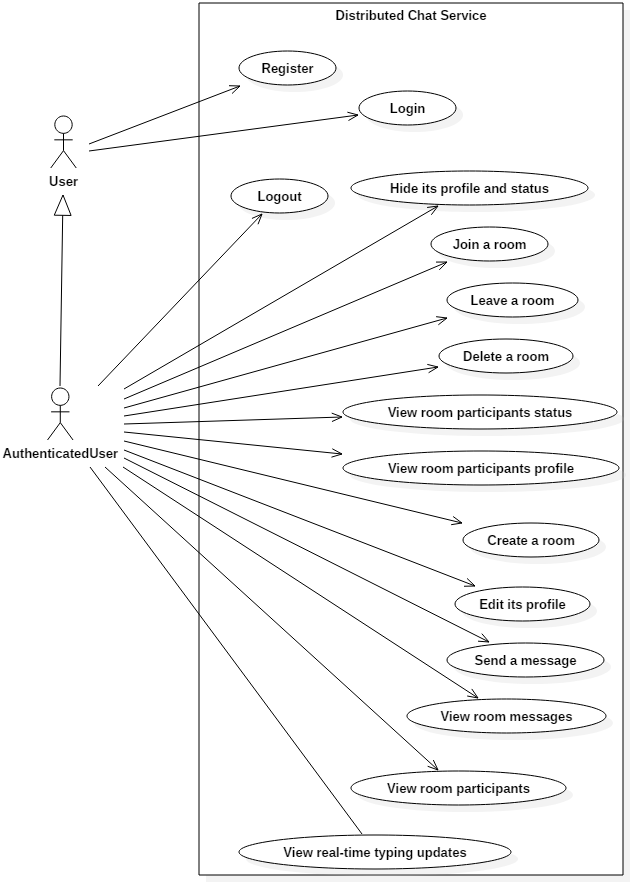
\includegraphics[width=\linewidth, keepaspectratio]{images/UseCaseDiagram.png}
  \caption{Diagramma dei casi d'uso.}
  \label{fig: use-cases}
\end{figure}

\subsection{Unione ad una stanza ed uscita}
L'unione dell'utente ad una stanza comporta la possibilità di visualizzare i messaggi in essa contenuta (anche precedenti al \textit{join} dell'utente), di inviare messaggi e di visualizzare le informazioni sulla stanza (numero, nome e data di join dei partecipanti). È possibile uscire in qualsiasi momento da una stanza a cui ci si era uniti.

\subsection{Eliminazione di una stanza}
È possibile, per il suo creatore, eliminare una stanza indipendentemente dal numero di messaggi e di partecipanti che contiene in un certo momento.

\subsection{Visualizzazione dello stato degli utenti}
Un partecipante ad una stanza può visualizzare lo stato degli altri partecipanti (a meno che lo stato da visualizzare appartenga ad un utente invisibile). Per \textit{stato} si intende l'effettiva \textit{connessione} al servizio di chat in un certo periodo temporale.

\subsection{Visualizzazione e modifica del profilo utente}
Un partecipante ad una stanza può visualizzare il profilo utente degli altri partecipanti (a meno che il profilo da visualizzare appartenga ad un utente invisibile). Il profilo utente è modificabile tramite apposita schermata e comprende: nome utente, nome, biografia e flag di invisibilità. 

\subsection{Aggiornamento real-time sullo stato di scrittura}
Nel momento in cui un utente scrive un messaggio all'interno di una stanza, allora agli utenti che partecipano alla stessa stanza verrà visualizzato il fatto che quell'utente sta digitando.

\subsection{Ricerca di una stanza per nome}
Sarà presente un'apposita schermata di ricerca di una stanza. La ricerca avviene digitando il nome della stanza da trovare.
Nel momento in cui l'utente inizia a digitare, verranno visualizzate tutte le stanze che contengono nel proprio nome la stringa digitata.
Successivamente, sarà possibile effettuare il \textit{join} alla stanza semplicemente cliccando sul suo nome.

\subsection{Offuscamento del proprio stato agli altri utenti}
Tramite la modifica del proprio profilo utente, è possibile impostare un \textit{flag di invisibilità}. Se tale flag è attivo, il proprio profilo ed il proprio stato non saranno visibili da altri utenti. Inoltre, non sarà possibile, per l'utente invisibile, visualizzare lo stato e profilo degli altri utenti.

\section{Requisiti non funzionali}
L'unico requisito non funzionale del sistema è la \textbf{sicurezza del sistema di interazione} tra i componenti del sistema, in particolare del meccanismo di autenticazione. Il sistema di autenticazione dovrà:
    \begin{itemize}
        \item Permettere la registrazione, inserendo \textit{username} e \textit{password}, 	rilasciando un \textit{token} di autenticazione all'utente;
        \item Memorizzare in maniera persistente le informazioni inserite;
        \item Permettere la cancellazione di un utente, fornendo il suo \textit{token} di autenticazione;
        \item Permettere il login, inserendo \textit{username} e \textit{password}, rilasciando un \textit{token} di autenticazione all'utente;
        \item Permettere la validazione di un \textit{token} di autenticazione, ottenendo la descrizione dell'utente in risposta.
    \end{itemize}
\textit{Alcune interazioni (etichettate come protette) tra i componenti del sistema saranno eseguibili soltanto previa autenticazione}; quindi necessiteranno dell'invio, contestuale alla richiesta, di un token precedentemente rilasciato dal sistema di autenticazione.

\section{Requisiti di implementazione}
Per lo sviluppo del progetto sono stati definiti a priori i seguenti requisiti implementativi:

\begin{itemize}
    \item \textbf{Scala}: il linguaggio da utilizzare per lo sviluppo della maggior parte del progetto deve essere \textit{Scala}. Imponiamo questo requisito in quanto vogliamo sperimentare il paradigma funzionale, appreso nel corso di \textit{Paradigmi di programmazione e sviluppo}, ed i vantaggi di \textit{Scala} rispetto ai linguaggi studiati in corsi precedenti.
    
    \item \textbf{Vertx}: data la natura dell'applicazione, abbiamo scelto \textit{Vertx} come piattaforma scalabile, concorrente, non bloccante e distribuita su cui realizzare i servizi di \textit{back-end} del sistema. \textit{Vertx} permette di realizzare applicazioni reattive fornendo buone performance ed un consumo di risorse ridotto.
    
    \item \textbf{TDD}: dato l'utilizzo di una metodologia di sviluppo \textit{Agile} e la necessità, vista la complessità del sistema, di un uso intensivo di strumenti di test da affiancare al puro sviluppo di funzionalità, è stato deciso di applicare quando possibile un modello di sviluppo \textit{test-driven}. In questo modo è possibile:
    \begin{itemize}
        \item ottenere, dopo una prima stesura, un codice in gran parte già testato.
        \item verificare in maniera automatica se successive modifiche al codice comportano una perdita di correttezza.
        \item ottenere una specifica delle funzionalità che il software prodotto deve realizzare.
    \end{itemize} 

    \item \textbf{Angular}: per la realizzazione del \textit{front-end} della web application è stato scelto il framework \textit{Angular}. Quest'ultimo è stato progettato per fornire uno strumento facile e veloce per sviluppare applicazioni che girano su qualunque piattaforma, inclusi smartphone e tablet. Infatti, le applicazioni web in Angular, in combinazione con il toolkit open source \textit{Bootstrap} o \textit{Angular Material} sono naturalmente responsive, ossia il design del sito web si adatta in funzione alle dimensioni del dispositivo utilizzato.
    
    \item \textbf{MySQL}: la gestione della persistenza è stata realizzata attraverso un \textit{Database} \textit{MySQL} con relativo deployment su piattaforma online \textit{GearHost}. La scelta di tale piattaforma è stata condizionata dall'esigenza di reperire uno spazio di hosting gratuito.
    
\end{itemize}

\chapter{Design architetturale}

\section{Pattern architetturali}
L’architettura del sistema è una classica \textbf{Client-Server}. \\
La parte server è stata suddivisa in \textbf{microservizi RESTFul}, a basso coupling, per aumentare la modularità;
\\
Il lato Server è stato realizzato secondo i principi della \textbf{Clean Architecture}, un pattern architetturale utile per ottenere una buona separazione dei compiti. 
\\
Il client adopera inoltre un'architettura \textbf{Component-Based}.
\subsection{Clean Architecture}
Per ottenere la separazione dei compiti, tale architettura impone la suddivisione del codice in differenti strati: ogni strato
può conoscere, chiamare ed utilizzare solo gli strati più interni, imponendo così la \textit{Dependency Rule}: in tal modo i cambiamenti di codice in uno strato esterno non causano modifiche agli strati interni. La Dependency Rule permette, dunque, di creare un sistema 
intrinsecamente modificabile e testabile, con tutti i benefici che ciò comporta. Inoltre, seguendo il \textit{Single Responsability Principle} e
dipendendo solo da astrazioni, diventa semplice sostituire le implementazioni.
\\

\begin{figure}
  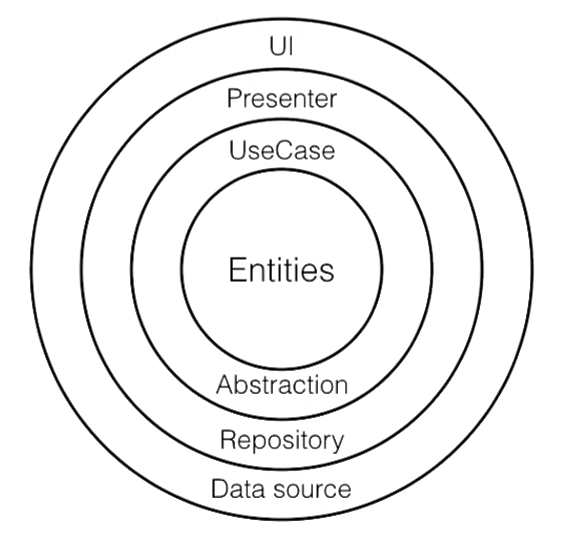
\includegraphics[scale=0.5, center]{images/CleanArchitectureLayersWhite.png}
  \caption{Rappresentazione della Dependency Rule e degli strati della Clean Architecture.}
  \label{fig: clean-architecture-layers-white}
\end{figure}

\begin{figure}
  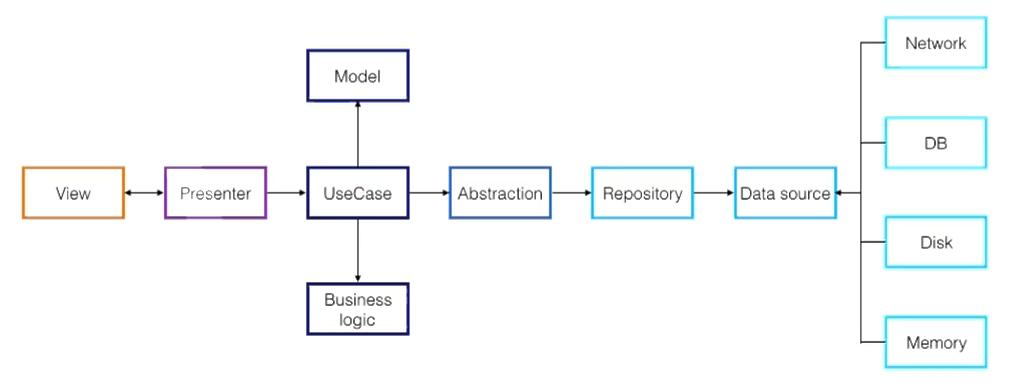
\includegraphics[width=\linewidth]{images/CleanArchitectureFlowWhite.png}
  \caption{Diagramma contenente tutti gli strati della Clean Architecture e le loro relazioni}
  \label{fig: clean-architecture-flow-white}
\end{figure}

Gli strati che compongono l'architettura sono i seguenti:
\begin{itemize}
    \item \textit{View}: prende gli eventi utente e li passa al presenter, mostrando inoltre i dati ricevuti dal presenter e permettendo
    azioni relative all'interfaccia grafica, come la gestione delle animazioni;
    \item \textit{Presenter}: fa da "middle man" tra la View e gli Use Cases; è il Presenter che formatta e passa i dati da visualizzare alla view e che gestisce gli eventi utente in arrivo dalla view, chiamando poi il giusto Use Case. Nel codice del Presenter non bisogna inserire nulla di relativo ad un singolo framework, poichè deve essere indipendente da essi;
    \item \textit{Use Case}: sono classi contenenti la logica necessaria per implementare un use case, ovvero uno specifico compito di business che l'utente cerca di portare a termine. Gli Use Case adoperano le classi di \textit{Model} e sfruttano uno o più abstractions. Dunque, gli Use Cases 
    ottengono i dati tramite le abstractions; a seguito di ciò essi usano le più appriopriate classi di business logic, per poi restituire un risultato, in modo asincrono, tramite un \textit{Subscriber} che il Presenter ha fornito;
    \item \textit{Abstraction}: astrazione per componenti specifici ad un framework;
    \item \textit{Repository}: un Repository è un data provider; al suo interno si sceglie quale \textit{Data Store} usare o, in caso se ne usi più di uno in contemporanea, se ne unisce i risultati (ad esempio si sceglie la sorgente dati che per prima restituisce il risultato). Il repository mappa in modo opportuno il risultato ottenuto, in modo che sia comprensibile dagli strati superiori, facendone in caso anche caching.
     \item \textit{Data Store}: è un'implementazione di una specifica sorgente dati; è dunque possibile realizzare multipli Data Source, uno per ogni tipologia di sorgente dati: Internet, Database, Disco Rigido, Memoria Centrale.
\end{itemize}
Il primo strato, ovvero la View, non è presente lato Server, poichè è il Client che se ne occupa.
\\
\\
La Clean Architecture permette di
ottenere i migliori risultati se usata assieme ai seguenti elementi, i quali sono stati da noi adottati:
\begin{itemize}
\item Un framework o tecnica di \textit{Dependency Injection}, per estrarre il codice di creazione delle dipendenze dalle classi, ottenendo codice più riusabile, testabile, leggibile e con maggiore separazione dei compiti. Qui la scelta è ricaduta sul \textit{Constructor Injection}, per la sua immediatezza nell'utilizzo;
\item \textit{Reactive Extensions}, per operare su sequenze di dati asincroni in modo dichiarativo e funzionale;
\item Un ampio uso delle lambdas, per ridurre la quantità di codice boilerplate.
\end{itemize}

\subsection{Microservizi}
Per architettura a microservizi si intende un'architettura formata da una collezione di servizi tra loro cooperanti e debolmente accoppiati, ovvero che non richiedono uno stack tecnologico specifico per l'interoperabilità, a meno delle principali tecnologie web. 
\\Il beneficio principale della scomposizione di un unico software monolite in più servizi è l'aumento di modularità, rendendo così più facile lo sviluppo: infatti, tale architettura permette di sviluppare e testare parti più piccole del sistema. Inoltre, permette lo sviluppo in maniera parallela e autonoma da parte di più teams. \\Infine, questa architettura rende più facile il raggiungimento di un buon livello di resilienza e scalabilità,  poichè, in caso di bisogno di replicazione, è possibile replicare la sola parte interessata, senza dover replicare l'intero monolite; infatti, spesso parti diverse del monolite hanno caratteristiche e necessità diverse, dunque è giusto permettere ad ogni parte di essere ridondata in un numero corretto di volte.

\subsection{Architettura del Client}
Il client è stato realizzato secondo un'architettura \textit{Component-Based}, che comprende i seguenti elementi:
\begin{itemize}
    \item \textit{Template}: definisce come renderizzare un componente, specificandone gli elementi grafici e i data bindings (mono o bidirezionali) dei relativi dati;
    \item \textit{Component}: è il codice che gescisce una sezione della vista, aggiornandone i dati e reagendo agli eventi, 
    chiamando, se necessario, uno o più \textit{Services}. Un Component è sempre associato ad un template. 
    I vari Component si distribuiscono ad albero, infatti ogni component può a sua volta contenere ulteriori Components, formando così la struttura della view.
    \item \textit{Service}: è un'ampia categoria che comprende un qualsiasi valore, funzione o funzionalità di cui l'applicazione ha bisogno.
\end{itemize}
Infine, è stato fatto abbondante uso di \textit{Dependency injection} sia nei Components sia nei Services, tramite i loro costruttori.

\section{Componenti del sistema distribuito}
Come già introdotto nella sezione precedente, il sistema vuole realizzare una \textit{Web Application} basata sul classico modello architetturale Client-Server.
Mentre la parte Client del sistema è rappresentata da un'unica applicazione monolitica, il sistema Server è stato scomposto in più componenti seguendo il modello a microservizi.
Dopo una prima fase di design del back-end del sistema, sono stati identificati 4 microservizi principali:
\begin{itemize}
    \item \textit{WebApp Service}
    \item \textit{User Service}
    \item \textit{Room Service}
    \item \textit{Authentication Service}
\end{itemize}
Inoltre è stato successivamente introdotto anche un \textit{servizio di Heartbeat} per permettere lo sviluppo della feature di visualizzazione dello stato effettivo di connessione al sistema di un utente.
Infine, viene descritta la struttura dei \textit{DB} utilizzati da ogni microservizio ai fini della persistenza delle informazioni.
Prima di descrivere ogni componente, viene successivamente definito il modello di riferimento delle entità di business del sistema. La definizione di tale modello infatti impatterà la struttura dei dati utilizzata da ogni componente.

\subsection{Model}
Prima di addentrarsi nell'analisi di ogni singolo componente del sistema distribuito, sono stati modellati i concetti di business principali tramite un diagramma delle classi \textit{UML}. Questa fase sarà utile poi per il design di ogni componente poichè permette di definire lo schema di base della struttura dei dati. Le entità di dominio e le relative associazioni sono espresse in Figura \ref{fig:model-class-diagram}.
\begin{figure}
  \centering
  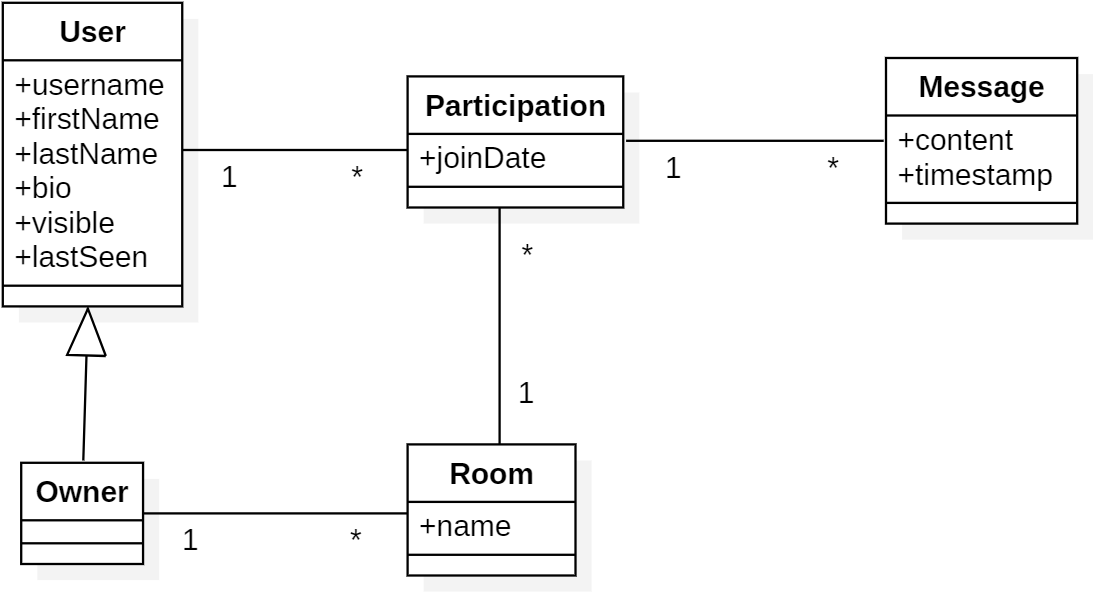
\includegraphics[height=15cm, width=12cm,
		keepaspectratio]{images/ModelClassDiagram.png}
  \caption{Diagramma delle classi delle entità di business.}
  \label{fig:model-class-diagram}
\end{figure}

\subsection{Web Client}
Rappresenta la parte del sistema utilizzabile dall'utente tramite un browser. Questo componente permette la visualizzazione delle schermate tramite le quali l'utente può interagire col sistema ed effettuare tutte le operazioni di business definite in fase di analisi del problema. Il \textit{Web Client} interagisce con il \textit{Server} sia in maniera \textit{pull} sia in maniera \textit{push}: questa duplice modalità di interazione permette di creare un sito web reattivo ai cambiamenti in maniera efficiente. Non vi è infatti, la necessità di effettuare \textit{polling} sul server per verificare se i dati sono stati aggiornati.
Nelle seguenti sottosezioni vengono definiti i componenti del sistema \textit{Client} considerando le astrazioni fornite dal framework \textit{Angular}.
\subsubsection{Components}
I principali componenti \textit{Angular} del \textit{front-end} identificati sono:
\begin{itemize}
    \item \textit{\textbf{Registration}}: incapsula la grafica della schermata di registrazione di un utente e la logica di controllo degli eventi scatenati dalla relativa interfaccia.
    \item \textit{\textbf{Login}}: incapsula la grafica della schermata di login e la logica di controllo degli eventi scatenati dalla relativa interfaccia.
    \item \textit{\textbf{Add-room}}: incapsula la grafica della schermata di creazione di una stanza e la logica di controllo degli eventi scatenati dalla relativa interfaccia.
    \item \textit{\textbf{Edit-profile}}: incapsula la grafica della schermata di \textit{editing} del proprio profilo utente, la logica di controllo degli eventi scatenati dalla relativa interfaccia e l'attivazione del recupero delle informazioni dell'utente corrente.
    \item \textit{\textbf{Room-info}}: incapsula la grafica della schermata di visualizzazione delle informazioni di una stanza, la logica di controllo degli eventi scatenati dalla relativa interfaccia e l'attivazione del recupero delle informazioni della stanza selezionata.
    \item \textit{\textbf{Rooms}}: incapsula la grafica della lista delle stanze a cui l'utente si è unito, la logica di controllo degli eventi scatenati dalla relativa interfaccia e l'attivazione del recupero delle stanze.
    \item \textit{\textbf{Search-rooms}}: incapsula la grafica della lista delle stanze ricercate, la logica di controllo degli eventi scatenati dalla relativa interfaccia e l'attivazione del recupero delle stanze. 
    \item \textit{\textbf{Sidebar}}: incapsula la grafica della schermata di visualizzazione delle stanze cercate o a cui l'utente si è unito e la logica di controllo degli eventi scatenati dalla relativa interfaccia.
    \item \textit{\textbf{Top-navbar}}: incapsula la grafica della barra di navigazione e la logica di controllo degli eventi scatenati dalla relativa interfaccia.
    \item \textit{\textbf{User-profile}}: incapsula la grafica della schermata di visualizzazione del profilo di un utente e l'attivazione del recupero delle informazioni sull'utente visualizzato.
\end{itemize}
\subsubsection{Services}
I servizi \textit{Angular} identificati sono:
\begin{itemize}
    \item \textit{\textbf{Authentication}}: mantiene il riferimento all'utente che si è autenticato e fornisce le funzionalità di \textit{login}, \textit{registrazione}, \textit{logout}.
    \item \textit{\textbf{Chat}}: permette di effettuare le principali chiamate, riguardanti la \textit{Chat}, al \textit{Server} e di intercettarne le relative risposte in maniera asincrona. 
    \item \textit{\textbf{User}}: offre le funzionalità di recupero/modifica del profilo utente e permette di aggiornare le informazioni sullo stato di connessione del \textit{Client}.
    \item \textit{\textbf{Event-bus}}: permette di utilizzare l'\textit{Event Bus} di \textit{Vertx} per interagire in maniera non bloccante secondo il modello \textit{publish-subscribe}. Viene utilizzato per intercettare gli eventi asincroni provenienti dal \textit{Server}. 
\end{itemize}

\subsubsection{Template}
Il template di base del front-end è la versione di \href{https://startangular.com/product/sb-admin-material/}{\textit{\underline{SB Admin}}} realizzata tramite componenti dell'UI framework \textit{Angular Material}. Sono stati utilizzati alcuni componenti del predetto template, editandoli in maniera opportuna per addattarli alle nostre esigenze grafiche. L'utilizzo di tale framework ha permesso di creare uno sito web accessibile e  naturalmente \textit{responsive}.
In Figura \ref{fig:sb-admin-login} viene mostrata la schermata iniziale del template precedentemente citato.
\begin{figure}
  \centering
  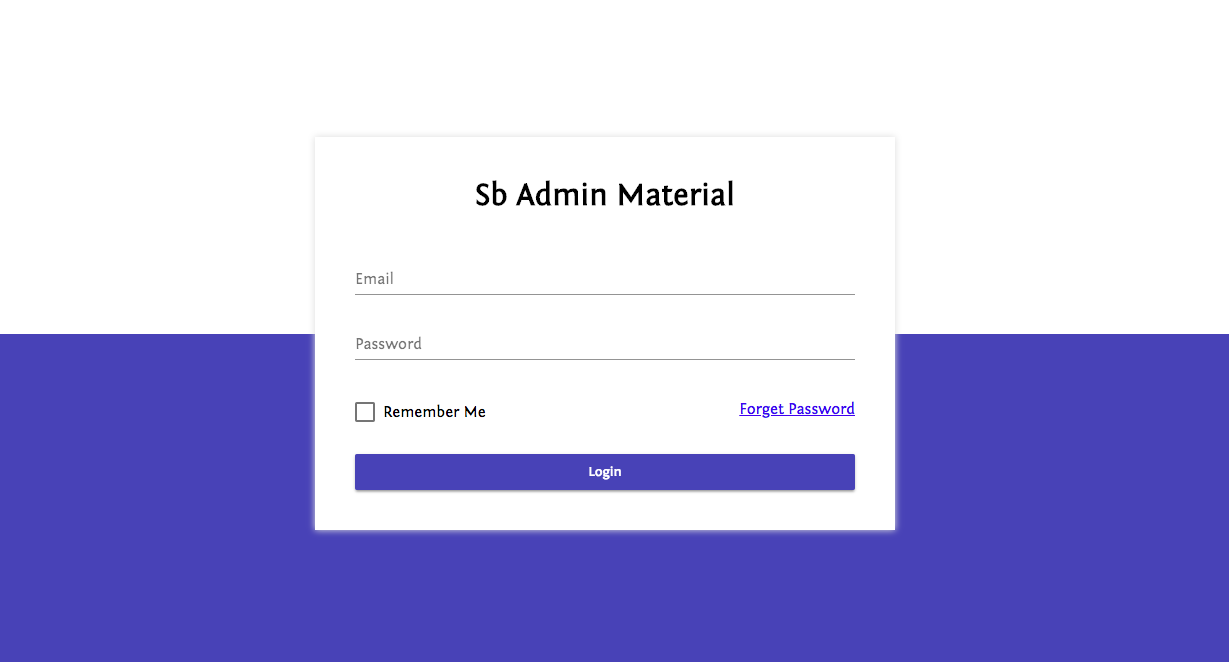
\includegraphics[height=15cm, width=12cm,
		keepaspectratio]{images/sb-admin.png}
  \caption{Schermata di login del template SB Admin realizzato tramite il framework UI \textit{Angular Material}.}
  \label{fig:sb-admin-login}
\end{figure}

\subsection{Web Server}
\subsubsection{Struttura}
Si elencano e descrivono di seguito, i componenti nei quali il \textit{Web Server} è stato scomposto. Come detto in precedenza infatti, questa parte del sistema è stata progettata secondo il modello a microservizi. 

\paragraph{WebApp Service}
Il \textit{WebApp Service} rappresenta il microservizio che gestisce l'interazione tra il client ed i restanti servizi di back-end. Il suo ruolo principale è quello di intercettare le richieste da parte dei client ed eseguire le operazioni necessarie per elaborare e restituire il relativo risultato. Nel perseguire il suo obiettivo il \textit{WebApp Service} tipicamente interagisce con uno o più microservizi di back-end.
La struttura del \textit{WebApp Service} è descritta tramite un diagramma UML delle classi in Figura \ref{fig:webapp-service-class-diagram}. In tale figura sono stati omessi alcuni dei casi d'uso per facilitare la lettura del resto del diagramma. Per completezza, si riporta la lista completa dei casi d'uso del \textit{WebApp Service} e le relative associazioni ai repositories:
\begin{itemize}
    \item \textit{\textbf{LoginUserUseCase}} $\longrightarrow$ \textit{AuthenticationRepository}, \textit{UserRepository}
    
    \item \textit{\textbf{RegisterUserUseCase}} $\longrightarrow$ \textit{AuthenticationRepository}, \textit{UserRepository}, \textit{RoomRepository}
    
    \item \textit{\textbf{LogoutUserUseCase}} $\longrightarrow$ \textit{AuthenticationRepository}, \textit{UserRepository}
    
    \item \textit{\textbf{JoinRoomUseCase}} $\longrightarrow$ \textit{AuthenticationRepository}, \textit{RoomRepository}
    
    \item \textit{\textbf{LeaveRoomUseCase}} $\longrightarrow$ \textit{AuthenticationRepository}, \textit{RoomRepository}
    
    \item \textit{\textbf{NotifyTypingInRoomUseCase}} $\longrightarrow$ \textit{AuthenticationRepository}
    
    \item \textit{\textbf{SendMessageUseCase}} $\longrightarrow$ \textit{AuthenticationRepository}, \textit{RoomRepository}
    
    \item \textit{\textbf{GetUserUseCase}} $\longrightarrow$ \textit{AuthenticationRepository}, \textit{UserRepository}
    
    \item \textit{\textbf{GetUserParticipationsUseCase}} $\longrightarrow$ \textit{AuthenticationRepository}, \textit{RoomRepository}
    
    \item \textit{\textbf{GetRoomsUseCase}} $\longrightarrow$ \textit{AuthenticationRepository}, \textit{RoomRepository}
    
    \item \textit{\textbf{GetRoomParticipationsUseCase}} $\longrightarrow$ \textit{AuthenticationRepository}, \textit{RoomRepository}
    
    \item \textit{\textbf{GetMessagesUseCase}} $\longrightarrow$ \textit{AuthenticationRepository}, \textit{RoomRepository}
    
    \item \textit{\textbf{EditUserUseCase}} $\longrightarrow$ \textit{AuthenticationRepository}, \textit{UserRepository}
    
    \item \textit{\textbf{DeleteRoomUseCase}} $\longrightarrow$ \textit{AuthenticationRepository}, \textit{RoomRepository}
    
    \item \textit{\textbf{CreateRoomUseCase}} $\longrightarrow$
    \textit{AuthenticationRepository}, \textit{RoomRepository}
    
    \item \textit{\textbf{UserOfflineUseCase}} $\longrightarrow$ \textit{UserRepository}
\end{itemize}

\begin{figure}
  \centering
  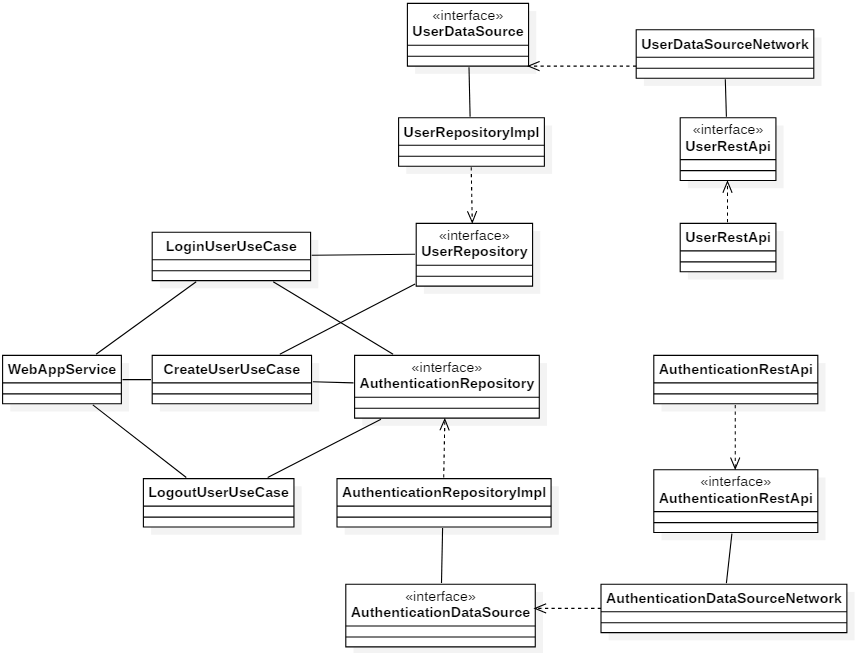
\includegraphics[height=15cm, width=12cm,
		keepaspectratio]{images/WepAppServiceClassDiagram.png}
  \caption{Diagramma delle classi dell'\textit{WebApp Service} (alcuni casi d'uso sono stati omessi per facilitare la lettura dello schema).}
  \label{fig:webapp-service-class-diagram}
\end{figure}

\paragraph{User Service}
Lo \textit{User Service} è il servizio che si occupa della persistenza delle informazioni degli utenti. Offre le classiche operazioni di lettura, scrittura ed aggiornamento sui dati utente. Esempi di operazioni che coinvolgono il servizio sono: reperimento della biografia utente, modifica del nome e cognome, ecc.
\begin{figure}
  \centering
  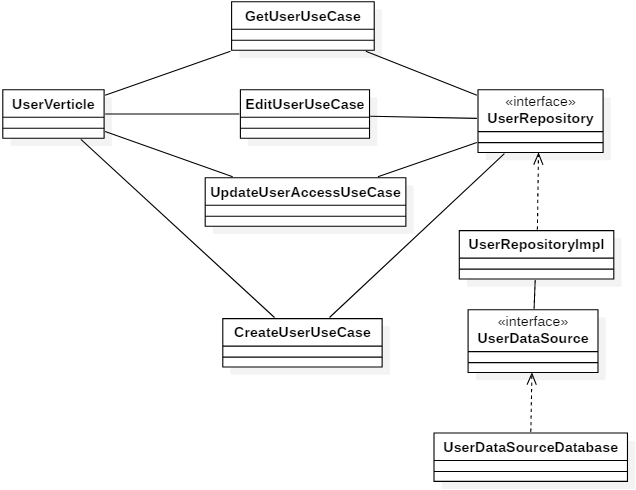
\includegraphics[height=15cm, width=12cm,
		keepaspectratio]{images/UserServiceClassDiagram.png}
  \caption{Diagramma delle classi dell'\textit{User Service}.}
  \label{fig:user-service-class-diagram}
\end{figure}

\paragraph{Room Service}
Il \textit{Room Service} è il servizio che si occupa della persistenza delle informazioni delle stanze. Offre le classiche operazioni di lettura, scrittura ed aggiornamento sui dati di una stanza. Operazioni tipiche che coinvolgono il Room Service sono ad esempio: reperimento dei messaggi e partecipanti di una stanza, invio di un messaggio, uscita dalla stanza, ecc.
La struttura di questo servizio è descritta dal diagramma delle classi in Figura \ref{fig:room-service-class-diagram}.
In tale figura sono stati omessi alcuni dei casi d'uso per facilitare la lettura del resto del diagramma. Per completezza, si riporta la lista completa dei casi d'uso del \textit{Room Service}:
\begin{itemize}
    \item \textbf{\textit{GetRoomsUseCase}}
    \item \textbf{\textit{SendMessageUseCase}}
    \item \textbf{\textit{DeleteRoomUseCase}}
    \item \textbf{\textit{LeaveRoomUseCase}}
    \item \textbf{\textit{JoinRoomUseCase}}
    \item \textbf{\textit{GetMessagesUseCase}}
    \item \textbf{\textit{CreateRoomUseCase}}
    \item \textbf{\textit{GetUserParticipationsUseCase}}
    \item \textbf{\textit{GetRoomParticipationsUseCase}}
    \item \textbf{\textit{CreateUserUseCase}}
\end{itemize}
\begin{figure}
    \centering
  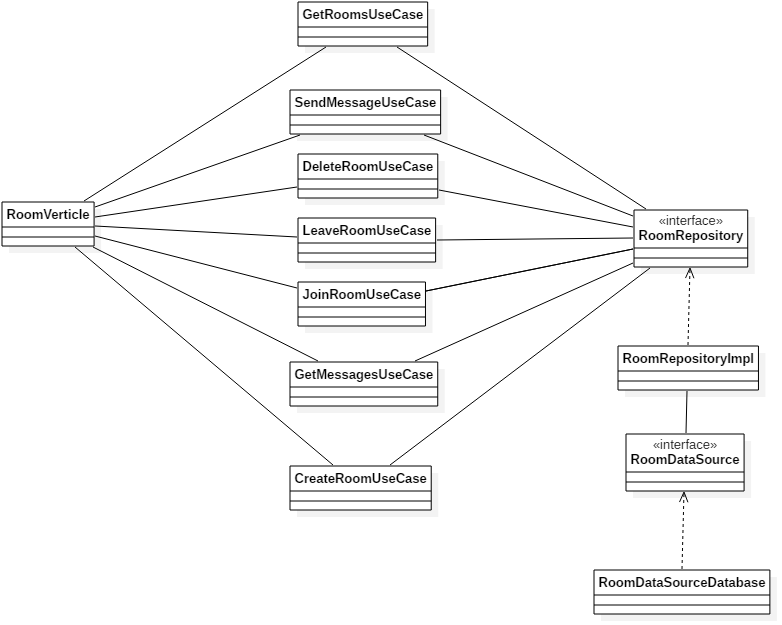
\includegraphics[height=15cm, width=12cm,
		keepaspectratio]{images/RoomServiceClassDiagram.png}
  \caption{Diagramma delle classi del \textit{Room Service} (alcuni casi d’uso sono stati omessi per facilitare la lettura dello schema).}
  \label{fig:room-service-class-diagram}
\end{figure}

\paragraph{Authentication Service}
L' \textit{Authentication Service} è il servizio che si occupa della gestione dell'autenticazione dell'utente e della protezione delle rotte di navigazione per le quali bisogna essere loggato per accedervi. Gestisce la persistenza delle credenziali degli utenti ed offre il servizio di creazione e validazione dei \textit{token}.
La struttura di questo servizio è descritta dal diagramma delle classi in Figura \ref{fig:authentication-service-class-diagram}.
\begin{figure}
  \centering
  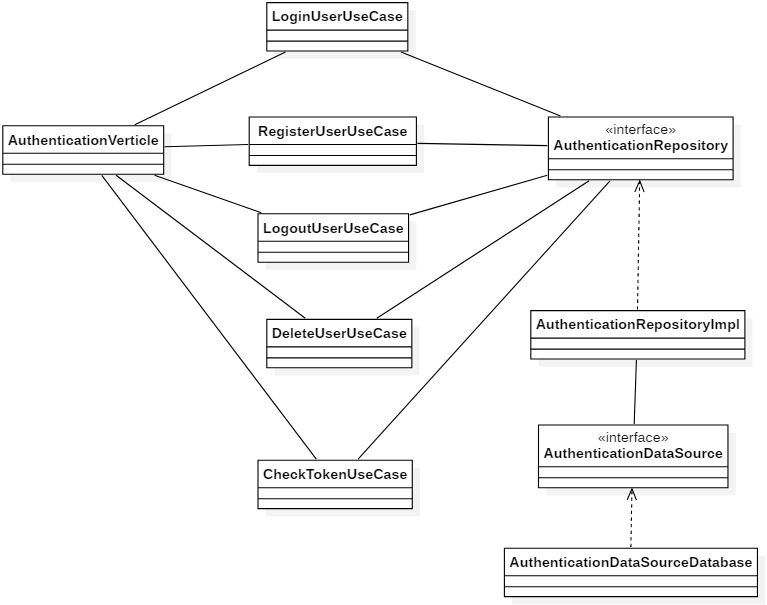
\includegraphics[height=15cm, width=12cm,
		keepaspectratio]{images/AuthenticationServiceClassDiagram.png}
  \caption{Diagramma delle classi dell'\textit{Authentication Service}.}
  \label{fig:authentication-service-class-diagram}
\end{figure}

\paragraph{Heartbeat Service}
L'\textit{Heartbeat Service} è il microservizio che si occupa di monitorare lo stato del client. Questo servizio monitora periodicamente i client connessi al sistema verificando se sono ancora connessi. In questo modo il sistema \textit{Server} riuscirà ad inviare ai vari client le informazioni riguardo lo stato di altri utenti.

\subsubsection{Interazione}
In primo luogo, viene riportata la descrizione della gerarchia dei microservizi che ne regola l'interazione. Infine, vengono presentati alcuni scenari di interazione tra i componenti del sistema.
\paragraph{Gerarchia dei microservizi}
La radice della gerarchia dei microservizi è rappresentata dal \textit{WebApp Service}. Quest'ultimo servizio infatti, funge da entry-point del sistema \textit{Server} e quindi da collante tra \textit{Client} e \textit{Server} (il \textit{Client} contatta sempre il \textit{WebApp Service}).
Il \textit{WebApp Service} a sua volta comunicherà, a seconda della funzionalità richiesta, con il \textit{Room Service}, \textit{Authentication Service} e \textit{User Service}. I servizi \textit{Room} e \textit{User} presentano una dipendenza verso il servizio di \textit{Authentication} poichè per effettuare alcune operazioni è necessario essere autenticati; quindi l'Authentication Service dovrà prima validare il \textit{token} dell'utente richiedente. Come è possibile vedere in Figura \ref{fig:microservices-hierarchy}, il WebApp Service interagisce anche con un \textit{servizio di Heartbeat}. Quest'ultimo è stato pensato per verificare e restituire lo stato di connessione dei \textit{Client} alla \textit{Web Application}.

\begin{figure}
    \centering
  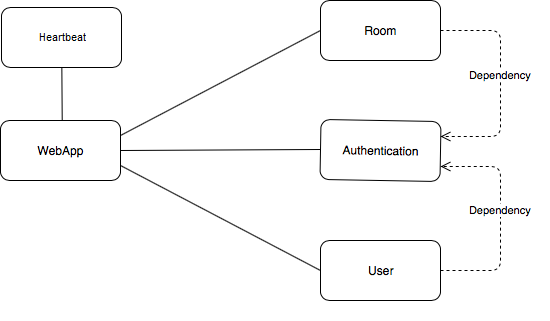
\includegraphics[width=\linewidth]{images/MicroserviceHierarchy_with_heartbeat.png}
  \caption{Gerarchia dei microservizi identificati per il back-end.}
  \label{fig:microservices-hierarchy}
\end{figure}

\subsection{Database}
Il modello scelto per il design del \textit{Database} è quello \textit{relazionale} poichè la natura dei dati è prevalentemente di tipo strutturata.
Per ogni microservizio che necessita di persistenza, è stato modellato uno \textit{schema E/R} che ne descriva la struttura dei dati. Secondo tale modello infatti, ogni servizio gestirà il proprio database che implementerà il relativo schema relazionale.
Di seguito vengono riportati gli schemi E/R dei servizi che utilizzano un \textit{Database}.

\subsubsection{Room Service DB}
Il database del \textit{Room Service} presenta 4 relazioni: 
\begin{itemize}
    \item \textit{User}: identificata dal solo \textit{username}. Uno \textit{User} può partecipare a più stanze e può essere il creatore di una stanza.
    \item \textit{Participation}: identificata dalla \textit{data di unione} ad una stanza, da un \textit{utente} e da una \textit{stanza}. Una partecipazione riguarda solamente un utente ed una stanza. Ad una partecipazione possono essere associati 1 o più messaggi.
    \item \textit{Message}: identificata da una partecipazione e da un timestamp. Presenta l'attributo \textit{content} che rappresenta il testo del messaggio. Ad ogni messaggio è associato una sola partecipazione.
    \item \textit{Room}: identificata dal solo \textit{nome della stanza}. Ogni stanza ha un solo creatore e può essere associata ad una o più partecipazioni.
\end{itemize}

\begin{figure}
    \centering
  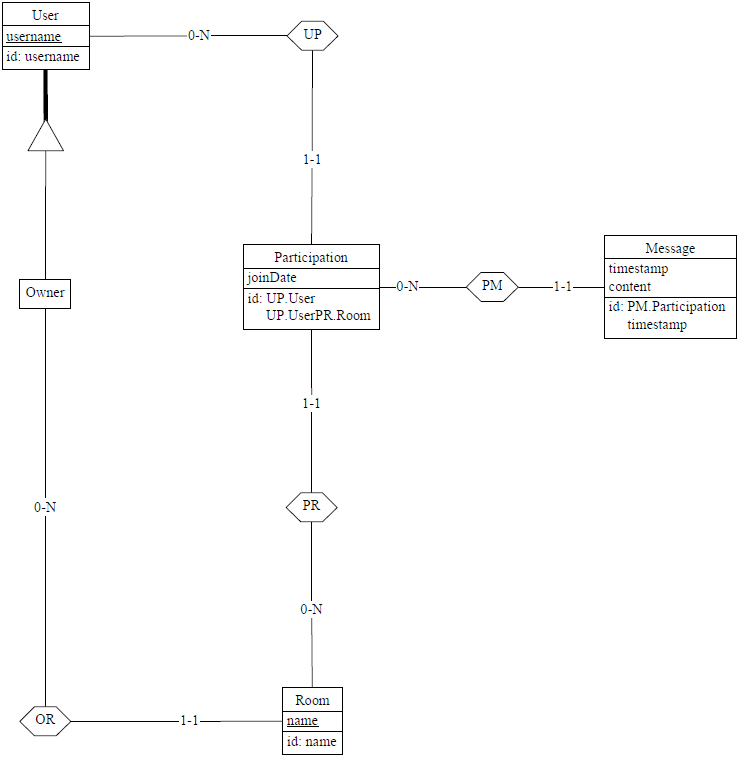
\includegraphics[height=15cm, width=12cm,
		keepaspectratio]{images/RoomServiceER.PNG}
  \caption{\textit{Schema E/R} del Database gestito dal \textit{Room Service}.}
  \label{fig:room-service-er-schema}
\end{figure}
\begin{figure}
    \centering
  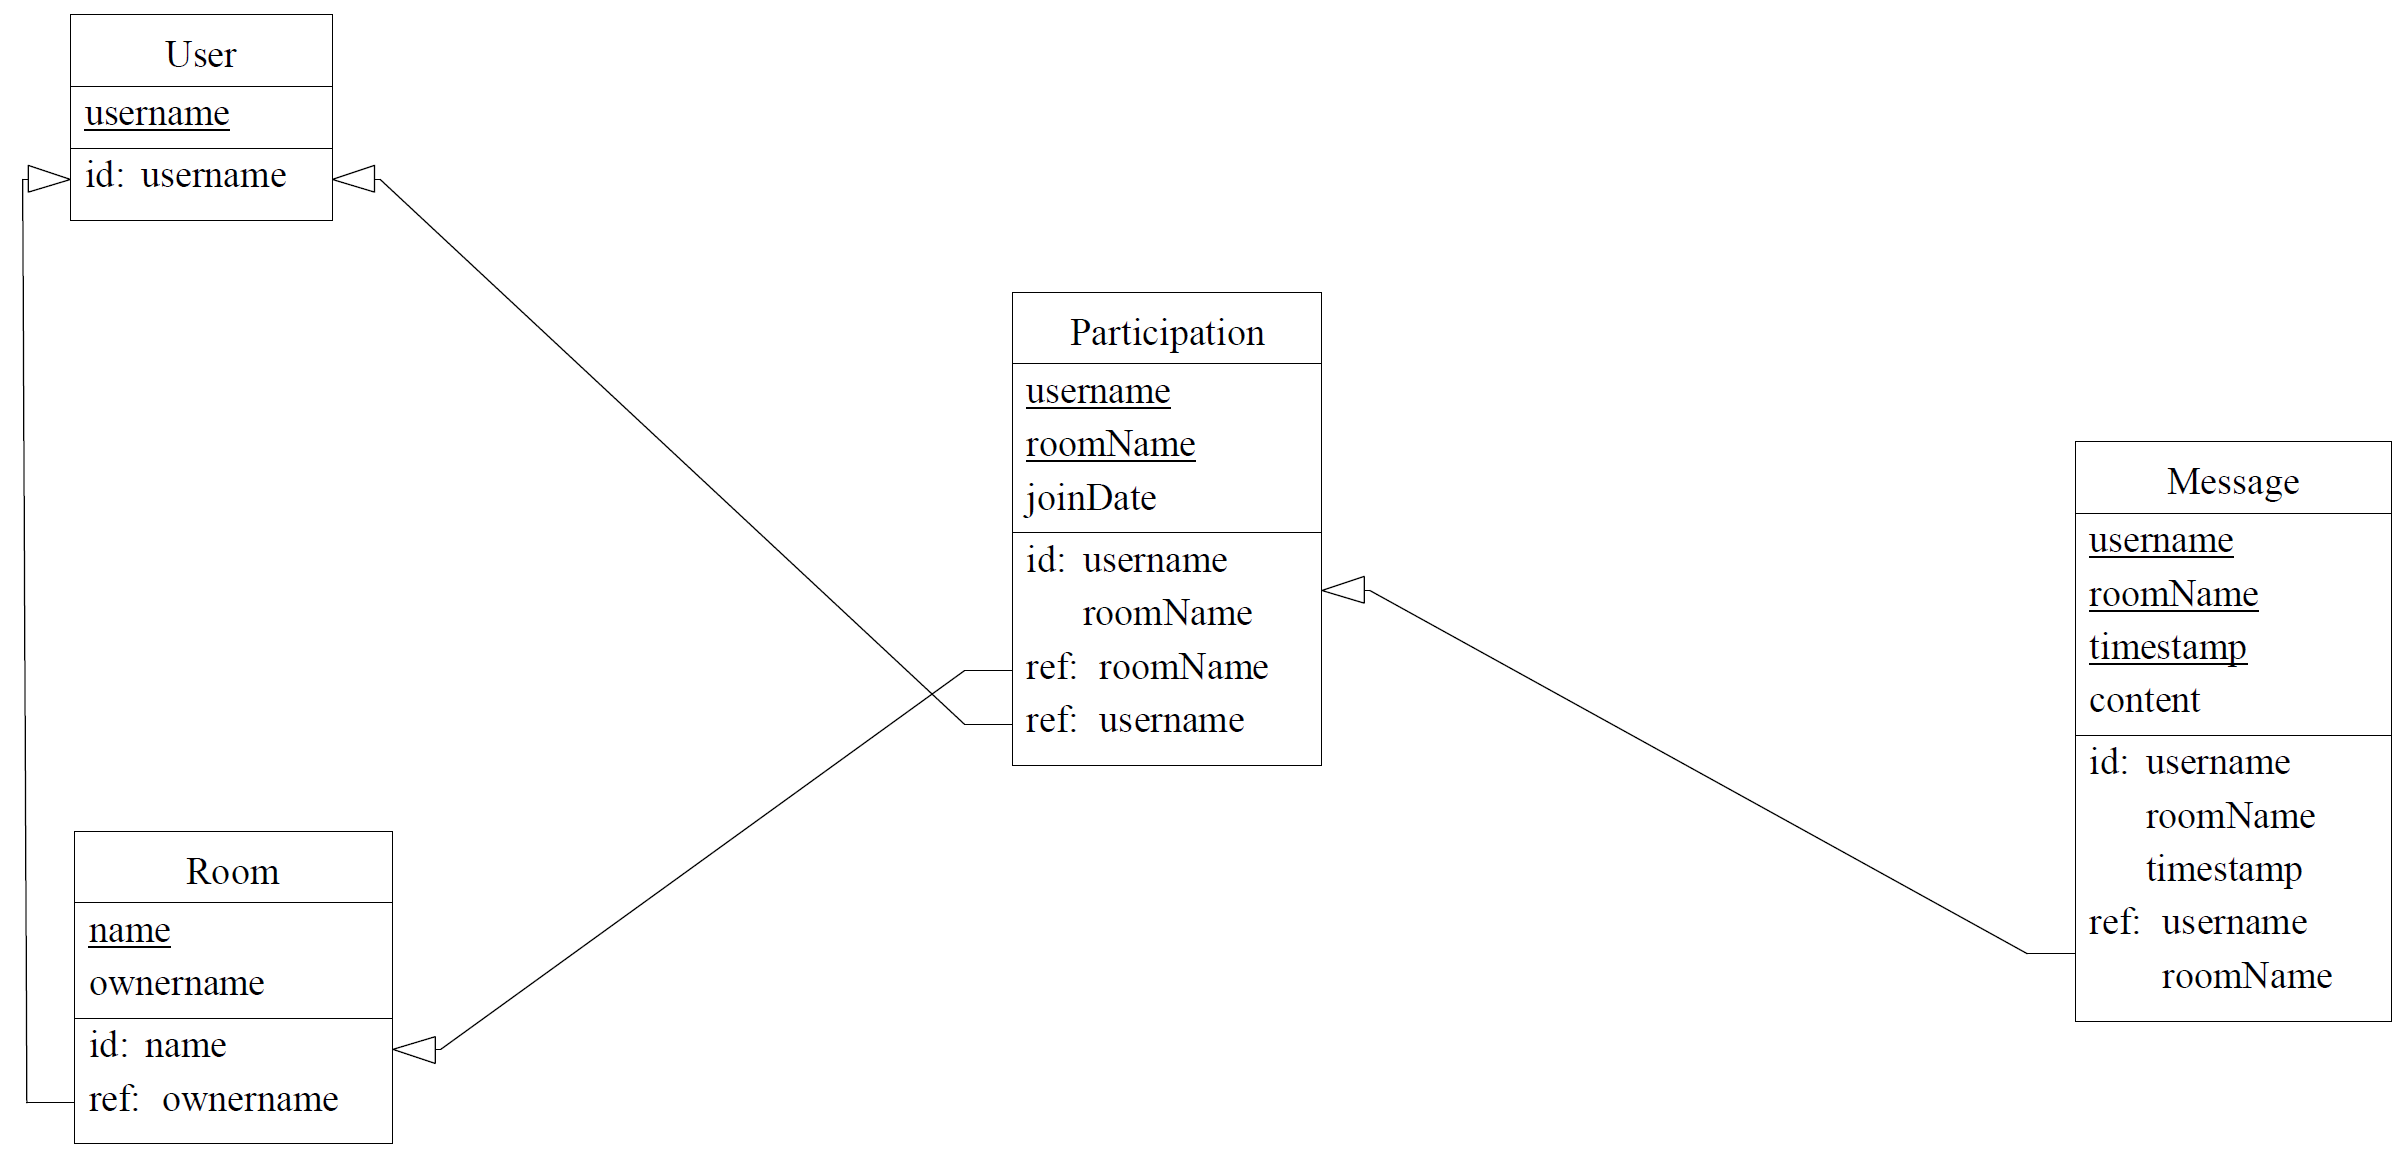
\includegraphics[height=15cm, width=12cm,
		keepaspectratio]{images/RoomServiceDBLogic.png}
  \caption{\textit{Schema logico} del Database gestito dal \textit{Room Service}.}
  \label{fig:room-service-logic-schema}
\end{figure}


\subsubsection{User Service DB}
Il database dello \textit{User Service} presenta una singola relazione \textit{User}. Essa è identificata dallo \textit{username} dell'utente ed è caratterizzata da: 
\begin{itemize}
    \item Nome
    \item Cognome
    \item Biografia
    \item Flag di visibilità
    \item Ultimo accesso
\end{itemize}
\begin{figure}
  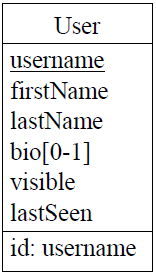
\includegraphics[width=5cm, height=3cm, keepaspectratio]{images/UserServiceER.PNG}
  \centering
  \caption{\textit{Schema E/R} del Database gestito dal \textit{User Service}.}
  \label{fig:user-service-er-schema}
\end{figure}

\newpage
\subsubsection{Authentication Service DB}
Il database dell'\textit{Authentication Service} presenta 2 relazioni: 
\begin{itemize}
    \item \textit{User}: identificato dallo username. È caratterizzata dall'attributo rappresentante la \textit{password} dell'utente. Ad ogni utente possono corrispondere uno o più token invalidi. Quest'ultimi infatti, hanno una scadenza e possono comunque essere invalidati dall'\textit{Authentication Service}. 
    \item \textit{InvalidToken}: identificata dalla stringa del token stesso. Presenta l'attributo corrispondente alla data di scadenza del token.
\end{itemize}

\begin{figure}
  \centering
  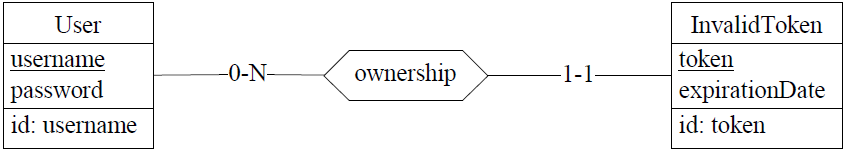
\includegraphics[height=15cm, width=12cm,
		keepaspectratio]{images/AuthenticationServiceER.PNG}
  \caption{\textit{Schema E/R} del Database gestito dall'\textit{Authentication Service}.}
  \label{fig:authentication-service-er-schema}
\end{figure}
\begin{figure}
  \centering
  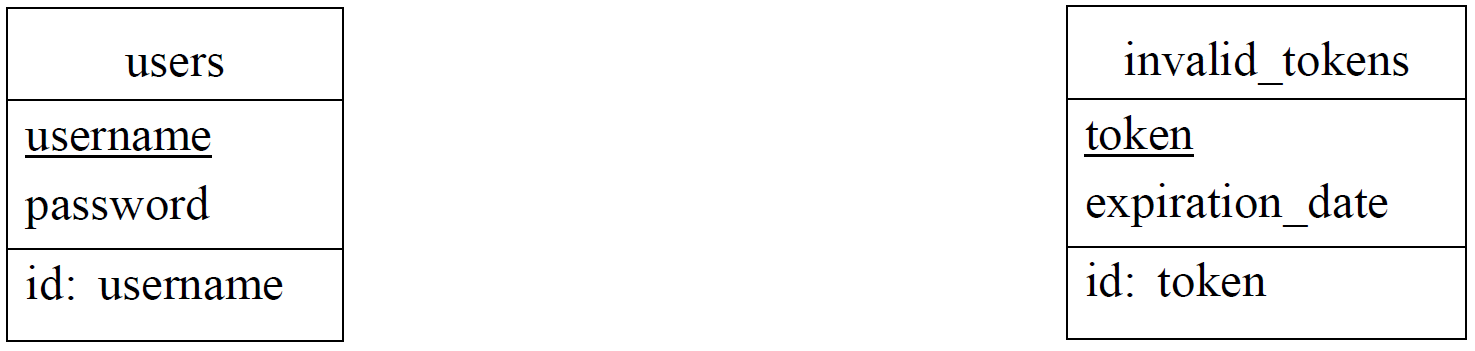
\includegraphics[height=15cm, width=12cm,
		keepaspectratio]{images/AuthenticationServiceDBLogic.PNG}
  \caption{Schema logico del Database gestito dall'\textit{Authentication Service}. L'associazione \textit{ownership} non è stata tradotta in chiave esterna della tabella \textit{invalid\_tokens} in quanto non necessaria; infatti il token intrinsecamente contiene l'informazione relativa allo \textit{username}.}
  \label{fig:authentication-service-logic-schema}
\end{figure}

\subsection{Esempi di interazione}
Riportiamo i diagrammi di sequenza riportanti alcuni degli scenari di interazione più interessanti che coinvologono i componenti core del sistema:
\begin{itemize}
    \item \textbf{Login di un utente} (Figura  \ref{fig:login-sequence-diagram})
        \begin{figure}
           \centering 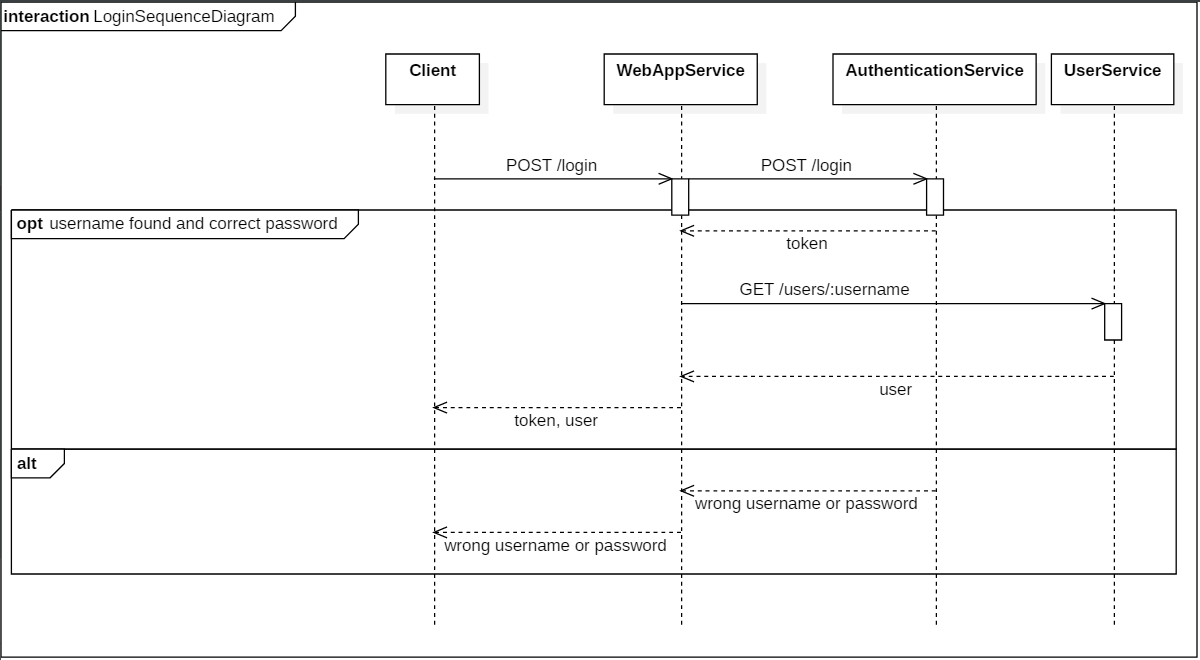
\includegraphics[width=\linewidth]{images/LoginSequenceDiagram.PNG}
            \caption{Diagramma di sequenza del login di un utente.}
            \label{fig:login-sequence-diagram}
        \end{figure}
        
    \item \textbf{Logout di un utente} (Figura  \ref{fig:logout-sequence-diagram})
        \begin{figure}
           \centering 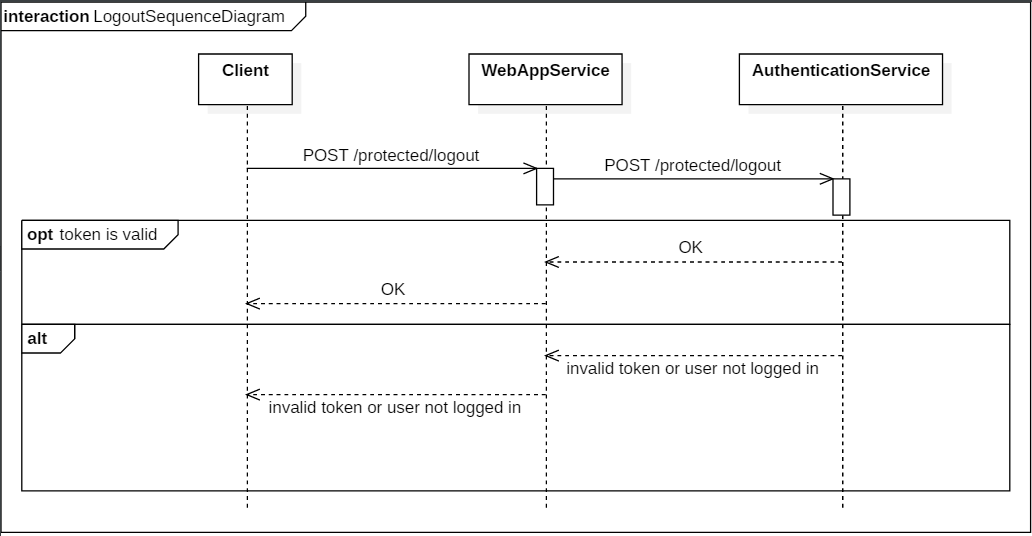
\includegraphics[width=\linewidth]{images/LogoutSequenceDiagram.PNG}
            \caption{Diagramma di sequenza del logout di un utente.}
            \label{fig:logout-sequence-diagram}
        \end{figure}
        
    \item \textbf{Registrazione di un utente} (Figura  \ref{fig:registration-sequence-diagram})
        \begin{figure}
           \centering 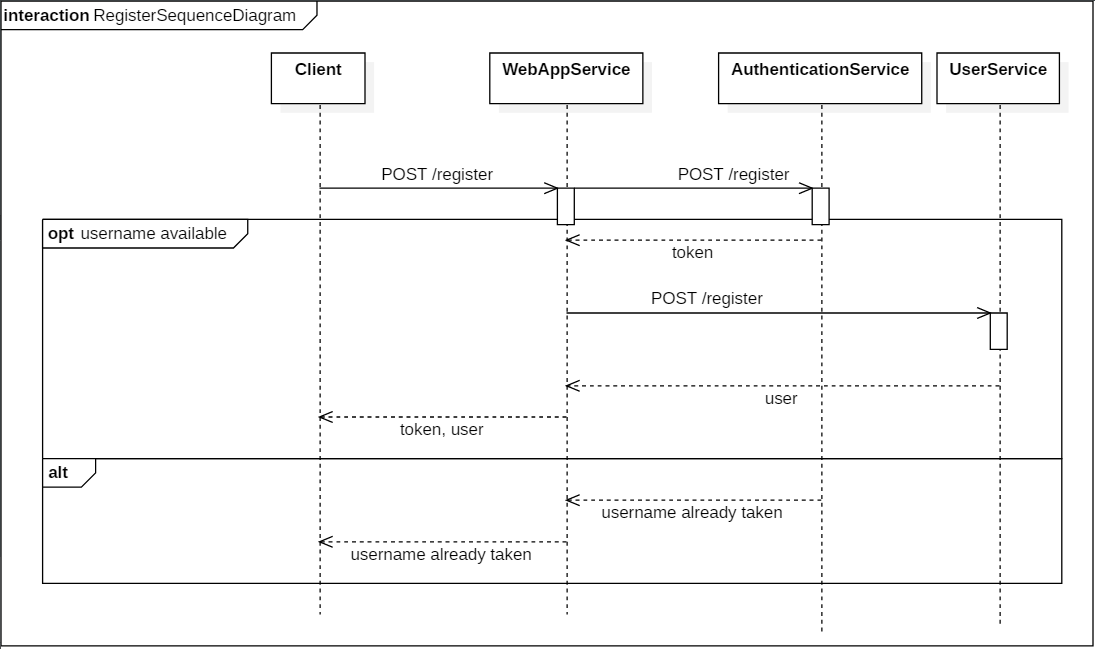
\includegraphics[width=\linewidth]{images/RegistrationSequenceDiagram.PNG}
            \caption{Diagramma di sequenza della registrazione di un utente.}
            \label{fig:registration-sequence-diagram}
        \end{figure}
        
    \item \textbf{Partecipazione ad una stanza} (Figura \ref{fig:join-room-sequence-diagram})
        \begin{figure}
           \centering 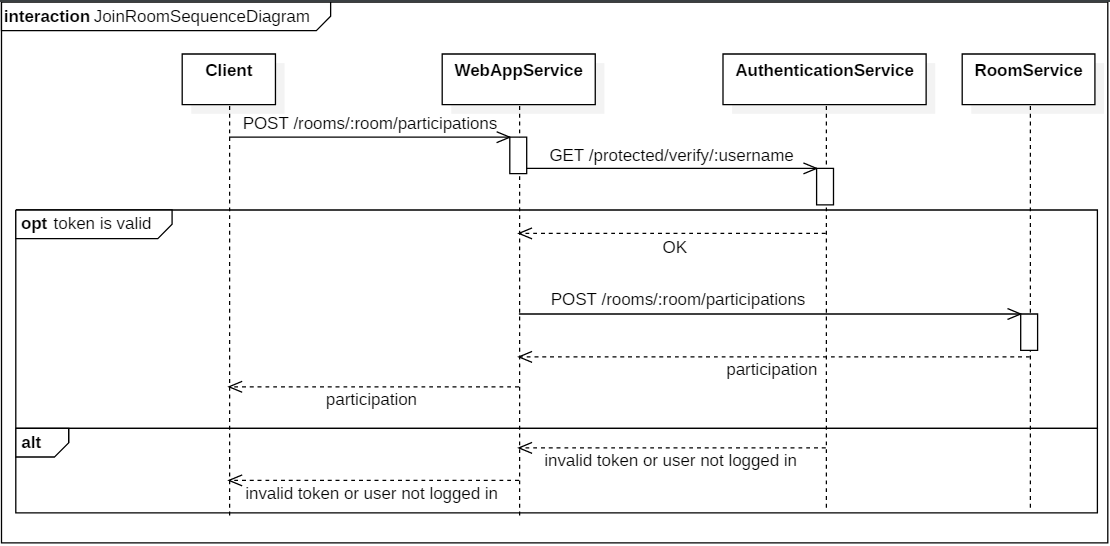
\includegraphics[width=\linewidth]{images/JoinRoomSequenceDiagram.PNG}
            \caption{Diagramma di sequenza dell'unione ad una stanza da parte di un utente.}
            \label{fig:join-room-sequence-diagram}
        \end{figure}
\end{itemize}


\section{Scelte tecnologiche cruciali ai fini architetturali}
\subsection{Vertx}
Vertx è un framework \textit{Event-Driven} poliglotta, utilizzabile per costruire applicazioni reattive sulla JVM. È inoltre non
bloccante, modulare e particolarmente veloce, favorendo così la concorrenza e la scalabilità. 
\\Il seguente è un elenco delle principali funzionalità e componenti sfruttati, resi disponibili da Vertx:
\begin{itemize}
    \item \textit{Verticle}: Vertx permette l'uso di un modello di concorrenza e deployment semplice, scalabile e Actor-like,
    realizzabile facendo uso dei Verticles. Un'applicazione Vertx è formata da uno o più Verticles, i quali possono essere \textit{Standard}, ovvero basati su un event loop, oppure \textit{Worker}, usando così uno dei thread dal Worker Pool, oppure \textit{Multi-threaded worker}, rendendo il codice eseguibile da più threads;
    \item \textit{EventBus}: è il "sistema nervoso" di Vertx, infatti permette diverse parti dell'applicazione di comunicare tra loro tramite scambio di messaggi asincrono, indipendentemente dal loro linguaggio e istanza Vertx in cui eseguono. L'EventBus supporta publish/subscribe e messaggi sia punto a punto sia request-response; esso è suddiviso in canali, potendo così registrare \textit{handlers} e pubblicare messaggi per uno specifico topic. È inoltre possibile creare un "ponte" con Javascript, rendendo dunque possibile l'uso dell'EventBus nei client Web: anche quest'ultima funzionalità è stata utilizzata;
    \item \textit{Clustering}: con questa funzionalità è possibile eseguire un insieme di istanze con capacità di alta disponibilità, dati distribuiti ed un Event Bus distribuito. Ciò è necessario per fare il deploy di Verticles su più istanze di Vertx, permettendo loro di collaborare;
    \item \textit{Vertx-Web}: è un insieme di funzionalità per la costruzione di applicazioni web, facilitando il routing, 
    il passaggio di parametri, la gestione di cookies e sessioni, ecc;
    \item \textit{Service Discovery}: questo componente fornisce un'infrastruttura per pubblicare e scoprire servizi e microservizi, i quali possono contenere risorse di varia natura;
    \item \textit{Vertx-Jdbc}: è un client che permette di interagire con ogni database compatibile con JDBC, usando
    un'API asincrona.
\end{itemize}
\begin{figure}
        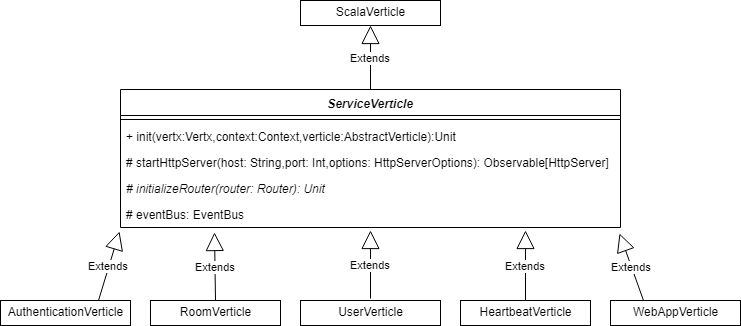
\includegraphics[scale=0.5, center]{images/VerticleClassDiagram.png}
        \caption{Diagramma delle classi che mostra le principali classi del progetto che estendono da \textit{Verticle}.}
        \label{fig:VerticleClassDiagram}
\end{figure}
\begin{figure}
        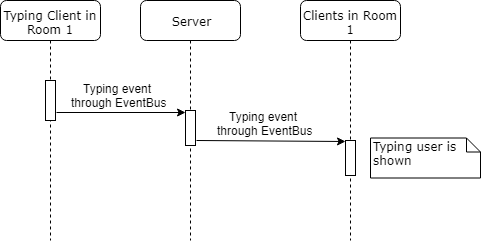
\includegraphics[scale=0.5, center]{images/EventBusSequenceDiagram.png}
        \caption{Diagramma di sequenza di un esempio di uso dell'\textit{EventBus}: l'aggiornamento in real-time dello stato di scrittura di un
        utente in una stanza.}
        \label{fig:EventBusSequenceDiagram}
\end{figure}
\begin{figure}
        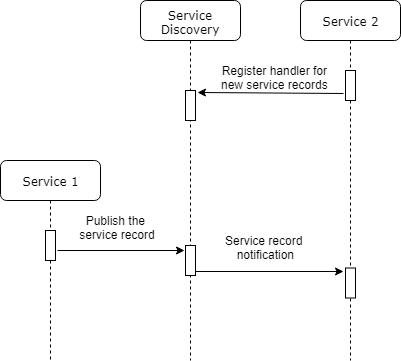
\includegraphics[scale=0.5, center]{images/ServiceDiscoverySequenceDiagram.png}
        \caption{Diagramma di sequenza di un esempio di uso del servizio di \textit{Service Discovery}.}
        \label{fig:ServiceDiscoverySequenceDiagram}
\end{figure}

Vertx è stato dunque scelto per le sue spiccate caratteristiche di velocità, scalabilità e capacità di fornire costrutti di alto livello utili e potenti.

\subsection{Angular}
Angular 2+ (o semplicemente Angular) è una piattaforma open source per lo sviluppo di applicazioni web con licenza \textit{MIT}, evoluzione di \textit{AngularJS}. E' stato sviluppato principalmente da Google, la sua prima release è avvenuta il 14 settembre 2016.
Il linguaggio di programmazione usato per \textit{Angular} è \textit{TypeScript}.

Le applicazioni sviluppate in Angular vengono eseguite interamente dal web browser dopo essere state scaricate dal web server. Questo comporta il risparmio di numerose richieste che dovrebbero essere altrimenti effettuate ogni volta che c'è una richiesta di azione da parte dell'utente. Il codice generato da Angular gira su tutti i principali web browser moderni quali ad esempio \textit{Chrome}, \textit{Microsoft Edge}, \textit{Opera}, \textit{Firefox}, \textit{Safari}, ecc.
I vantaggi dell'utilizzo di tale framework sono davvero considerevoli:
\begin{itemize}
    \item \textbf{TypeScript}: Le applicazioni \textit{Angular} sono costruite usando il linguaggio \textit{TypeScript}, un linguaggio costruito sopra JavaScript, che garantisce maggiore sicurezza in quanto supporta tipi (primitive, interfacce, ecc.) in fase di compilazione. Inoltre, aiuta a catturare ed eliminare gli errori in anticipo durante la scrittura del codice o l'esecuzione di attività di manutenzione.
    \item \textbf{UI espressa in modo dichiarativo} tramite l'uso di \textit{HTML}.
    \item \textbf{POJO}: Con Angular, non sono necessarie ulteriori funzioni getter e setter. Dato che ogni oggetto che usa è POJO (Plain Old JavaScript Object), che abilita la manipolazione degli oggetti fornendo tutte le funzionalità JavaScript convenzionali. È possibile rimuovere o aggiungere proprietà dagli oggetti, oltre a eseguire il loop su questi oggetti quando richiesto.
    \item \textbf{Pattern MVC incorporato}: lo sviluppatore \textit{Angular} non deve creare i classici blocchi previsti dall'architettura \textit{MVC} ma deve solo preoccuparsi di suddividere i componenti SW secondo i concetti forniti dal framework.
    \item \textbf{Struttura modulare}: realizzata tramite la divisione del SW in \textit{components}, \textit{services} e \textit{templates}. In Figura \ref{fig:angular-chat-service-dependencies-diagram} si può vedere un esempio di servizio \textit{Angular}. In particolare è stato scelto di rappresentare la struttura e le dipendenze del \textit{ChatService}. Si riporta, in Figura \ref{fig:angular-room-info-component-dependencies-diagram}, anche un esempio di un componente \textit{Angular}. Nello specifico, è stato rappresentato il componente \textit{room-info}, responsabile delle visualizzazione delle informazioni riguardanti una stanza.
    \begin{figure}
        \centering
        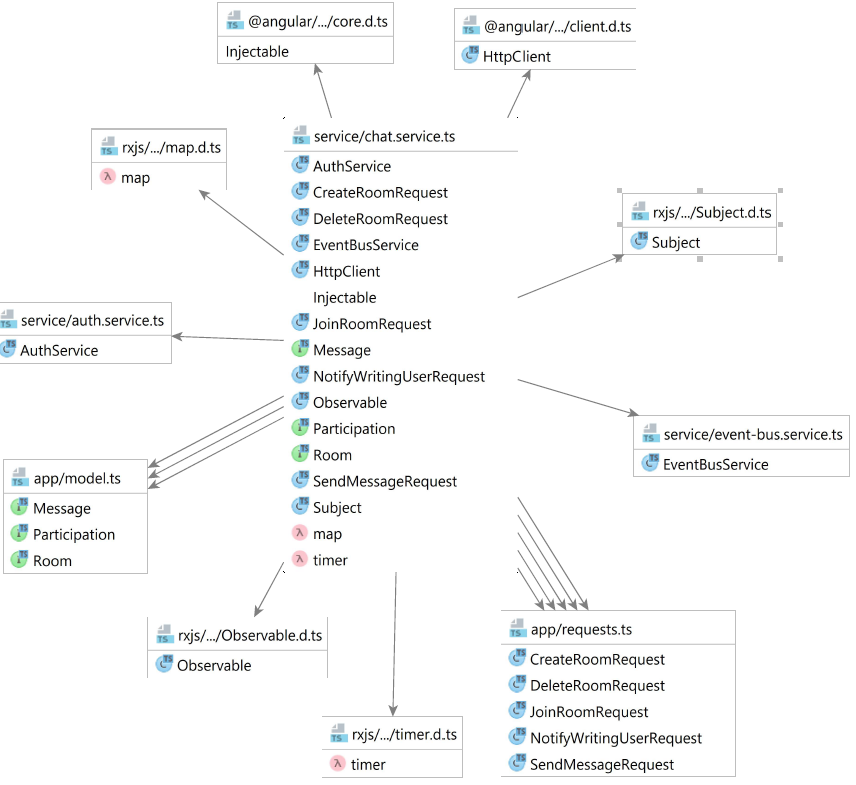
\includegraphics[height=15cm, width=12cm, keepaspectratio]{images/chat-service-dependencies.PNG}
        \caption{Diagramma delle dipendenze del servizio \textit{Angular} \textit{ChatService}.}
        \label{fig:angular-chat-service-dependencies-diagram}
    \end{figure}
    \begin{figure}
        \centering
        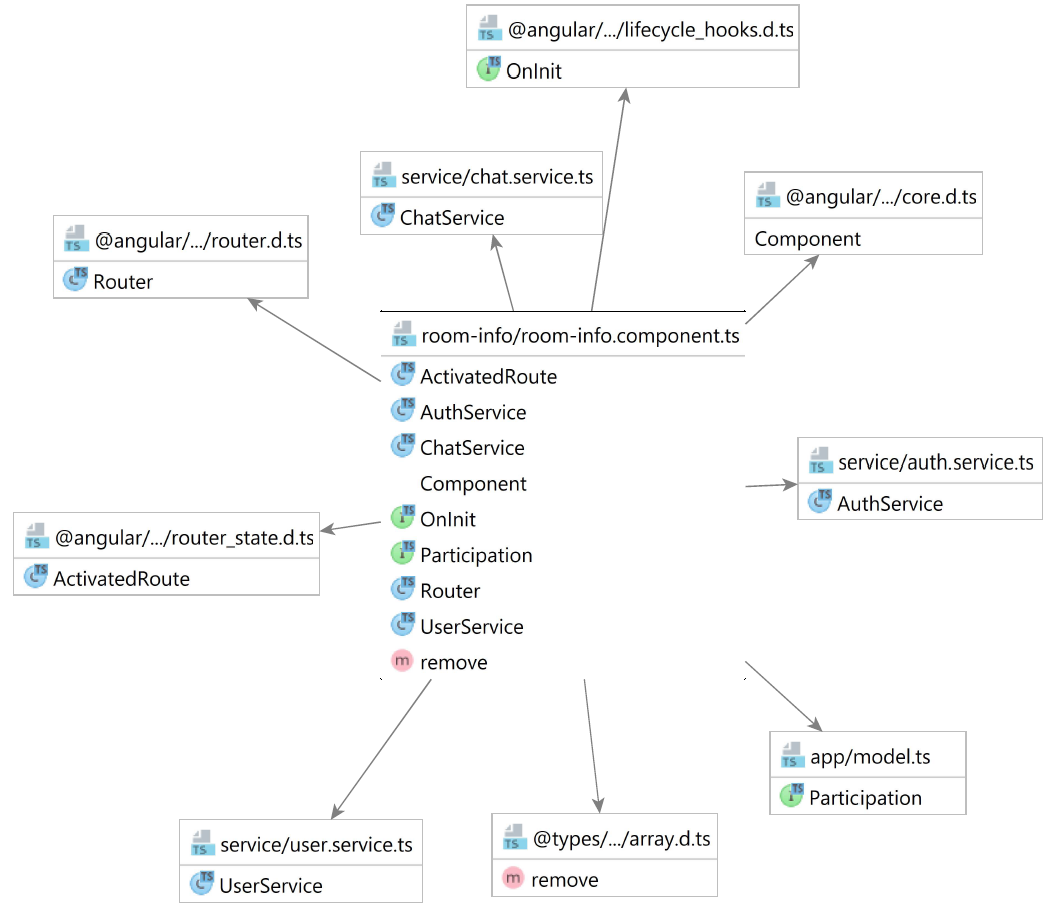
\includegraphics[height=15cm, width=12cm, keepaspectratio]{images/room-info-component-dependencies.png}
        \caption{Diagramma delle dipendenze del componente \textit{Angular} \textit{Room-info}.}
        \label{fig:angular-room-info-component-dependencies-diagram}
    \end{figure}
    \item \textbf{Consistenza del codice} 
        \begin{itemize}
         \item \textbf{Riusabilità}
         \item \textbf{Migliore leggibilità}
         \item \textbf{Facilità di manutenzione}
         \item \textbf{Unit-Testing semplificato}
        \end{itemize}
    \item \textbf{Performance}: in quanto \textit{Angular} mette a disposizione una modalità di deployment detta \textit{Production} nella quale esegue una serie di ottimizzazioni importanti (e.g. minificazione dei file css, js, ecc.).
\end{itemize}

\chapter{Design di Dettaglio}

In questo capitolo vengono analizzate le scelte operate a livello di design nel dettaglio. In particolare viene analizzata la struttura data a ciascuno dei servizi ed i principali pattern di progettazione adottati.

\section{Suddivisione in moduli}

Il nostro progetto è stato suddiviso in moduli in quanto permette un'organizzazione \textit{by-need} dei singoli moduli. Questo permette ad ogni modulo di includere come dipendenza solo i moduli di cui necessita, ottimizzando l'incapsulamento.

I moduli definiti sono:

\begin{itemize}
%
    \item \textit{Commons}: contiene tutte le parti di codice riutilizzate all'interno dei diversi moduli.
%
    \item \textit{Data Access}: contiene tutte le parti di codice riutilizzate per l'accesso (in lettura e scrittura) ad una base di dati relazionale.
%
    \item \textit{Exceptions}: contiene una rappresentazione di tutte le eccezioni di dominio e fornisce costrutti utili per la loro gestione.
%
    \item \textit{Interactors}:  contiene i costrutti comuni per la creazione di casi d'uso.
%
    \item \textit{Service Commons}: contiene i costrutti comuni per la creazione, pubblicazione e scoperta di servizi.
%
\end{itemize}

\section{Parti comuni}

In questa sezione vengono descritte le parti di codice comune che vengono riutilizzate all'interno di altri moduli.

\subsection{Commons}

All'interno del modulo \textit{Commons} sono state fattorizzate principalmente:

\begin{itemize}
%
    \item Alcune funzionalit\`a generiche:
    \begin{itemize}
%
        \item logging;
%
        \item lettura di file.
%
    \end{itemize}
%
    \item Funzionalit\`a per agevolare la trasformazione da oggetti descritti in formato \textit{JSON} a costrutti Scala.
%
    \item Funzionalit\`a per la conversione da costrutti di Vert.x a \texttt{Scheduler} RxScala e classi implicite per arricchire gli \texttt{Observable} RxScala con funzionalit\`a aggiuntive.
%
    \item Funzionalit\`a per convertire una chiamata asincrona ad un metodo fornito da Vert.x in un \texttt{Observable} RxScala, metodi di conversione e utilizzo del pattern  \textbf{Pimp my Library} per arricchire di nuove funzionalit\`a le classi \texttt{AsyncResult}, \texttt{EventBus} e \texttt{Json}.
%
    \item Funzionalit\`a per agevolare l'estrazione di parametri dal contesto di una richiesta HTTP e una classe implicita per estendere il costrutto \texttt{HttpServerResponse} di Vert.x.
%
    \item Altri costrutti pi\`u avanzati sono descritti in dettaglio nelle successive sotto-sezioni.
%
\end{itemize}

\begin{figure}[H]
  \centering
    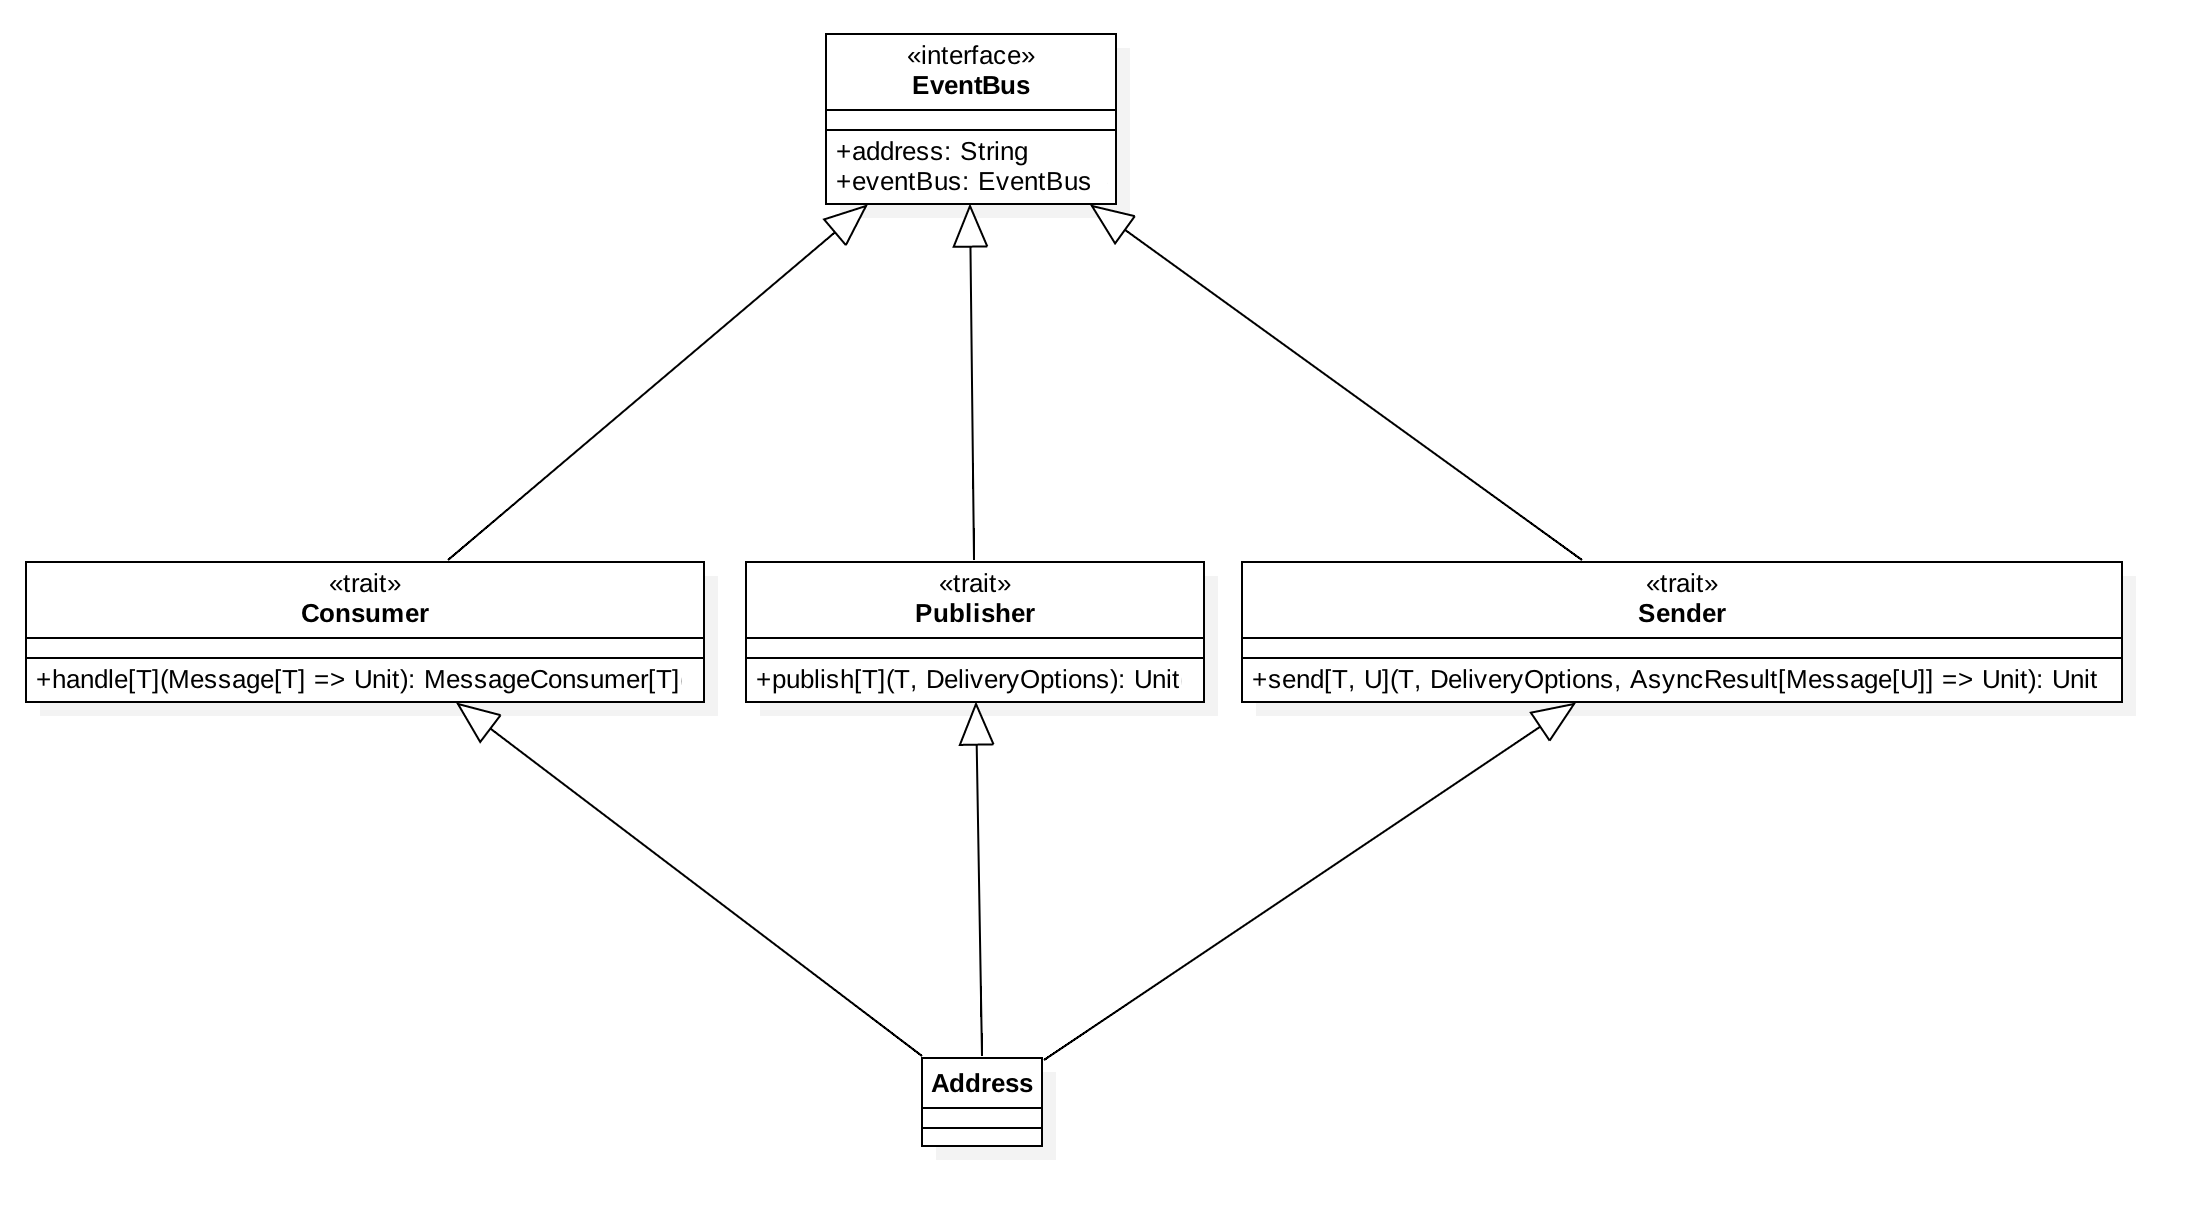
\includegraphics[width=\linewidth, height=\textheight, keepaspectratio]{AddressClassDiagram}
  \caption{Utilizzo del \textit{mix-in} per aggiungere funzionalit\`a alla classe \texttt{Address}.}
\end{figure}

\subsubsection{Validazione}

Per realizzare la validazione dell'input utente è stato utilizzato il pattern \textit{builder}.
%
La scelta di utilizzare questo pattern progettuale \`e legata al fatto che non \`e possibile determinare a priori quante (e quali) regole dovranno essere applicate per effettuare la validazione di un input.

La classe \texttt{ValidatorBuilder} \`e incaricata di gestire la costruzione di un oggetto \texttt{Validator}, per fare ciò \`o espone il metodo \texttt{addRule} che permette di aggiungere al builder un ulteriore regola di validazione.
%
\texttt{ValidatorBuilder} espone due overload del metodo \texttt{addRule}, il primo prende in input una regola da applicare, il secondo prende in input un predicato e un'eccezione da sollevare nel caso l'oggetto passato in input al validatore non sia soddisfatta.

Per la creazione di oggetti di tipo \texttt{Validator} \`e stato utilizzato il pattern \textit{Execute Around} che permette, tramite un espressione lambda, di eseguire un blocco di codice ed incapsulare all'interno del metodo eventuali operazioni di creazione e \textit{clean-up}.

\begin{figure}[H]
  \centering
    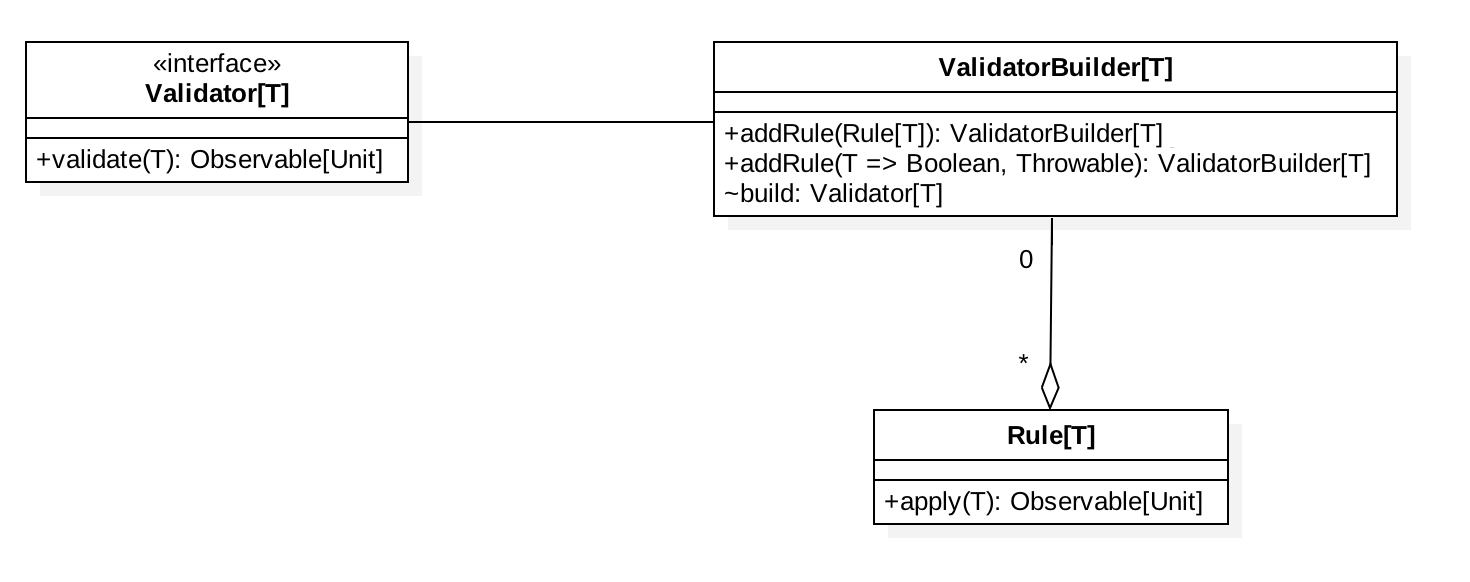
\includegraphics[width=\linewidth, height=\textheight, keepaspectratio]{ValidationClassDiagram}
  \caption{Diagramma delle classi per la classe per la costruzione di un \texttt{Validator}.}
\end{figure}

\subsubsection{Configurazione}

Per gestire la configurazione di oggetti complessi è stata utilizzata la classe \texttt{Configurator}, la quale permette di applicare in cascata un insieme di funzioni ad un'istanza passata in input.

\subsection{Data Access}

All'interno del modulo \textit{Data Access} sono state inserite tutte le parti di codice che sono state riutilizzate all'interno di altri moduli per semplificare l'interazione con la base di dati sottostante, inoltre espone alcune conversioni per agevolare la traduzione di tipi di dato Scala in tipi di dato interpretabili MySQL (nello specifico \texttt{Boolean} e \texttt{java.util.Date}).
%
Utilizzo del pattern \textbf{Pimp my Library} per arricchire la classe \texttt{ResultSet} aggiungendovi un metodo che permette di ottenere una rappresentazione JSON di ogni record restituito dall'interrogazione.

\subsection{Exceptions}

All'interno del modulo \textit{Exceptions} sono contenute tutte le possibili eccezioni che l'applicazione potrebbe sollevare. Fornisce metodi utili per la conversione delle eccezioni in oggetti JSON (e viceversa), oltre ad un metodo per determinare il tipo di errore HTTP a partire dall'eccezione sollevata.

\subsection{Interactors}

All'interno del modulo \textit{Interactors} sono contenuti i costrutti comuni per la creazione di casi d'uso.

La classe \texttt{UseCase}, classe padre di tutti i casi d'uso, sfrutta il pattern progettuale \textit{Template method} per raccogliere a fattor comune le modalit\`a di interazione e lasciare alle sottoclassi la definizione del comportamento.

\begin{figure}[H]
  \centering
    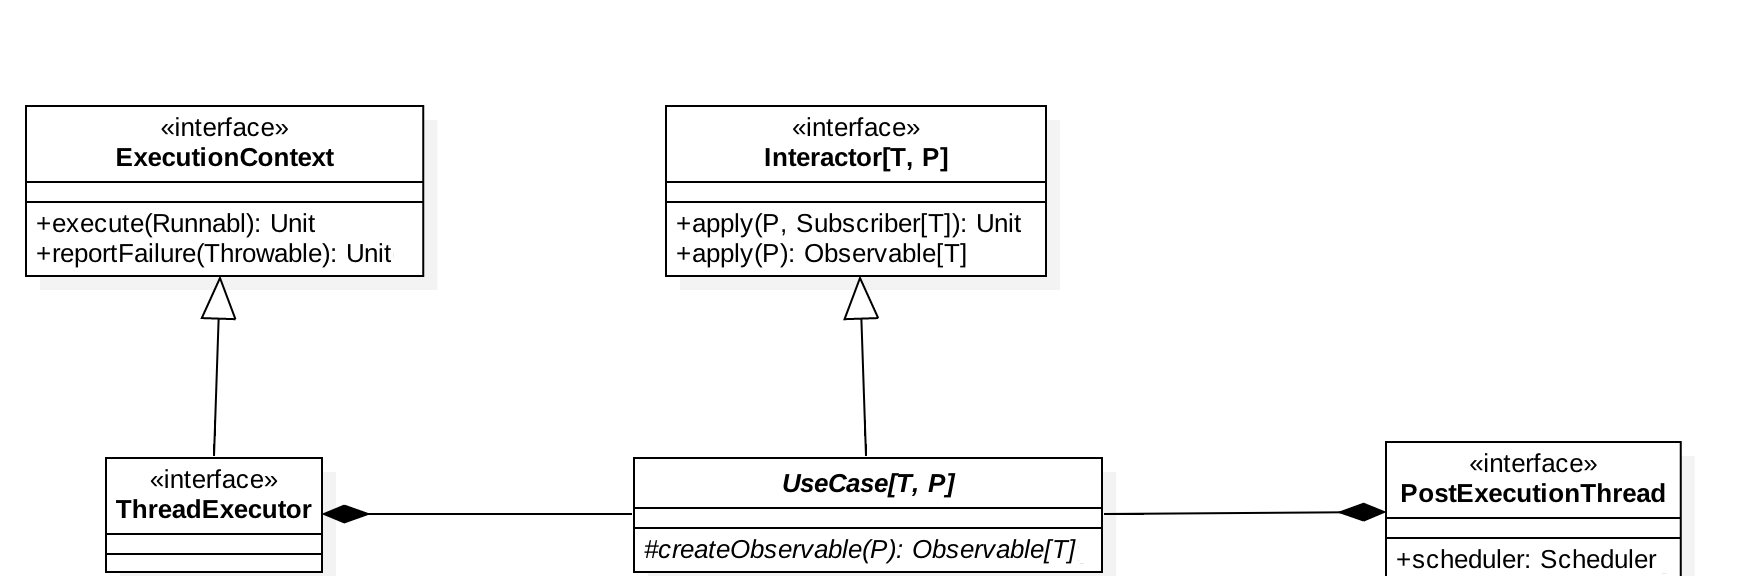
\includegraphics[width=\linewidth, height=\textheight, keepaspectratio]{UseCaseClassDiagram}
  \caption{Diagramma delle classi per la classe \texttt{UseCase}.}
\end{figure}

\subsection{Service Commons}

All'interno del modulo \textit{Service Commons} sono contenuti i costrutti comuni per la definizione, pubblicazione e scoperta di un servizio.

\`E utilizzato il pattern \textit{Template method} nella classe \texttt{ServiceVerticle} al fine di raccogliere a fattor comune le modalit\`a di inizializzazione del componente e demandare alle sottoclassi la definizione delle proprie rotte.

\section{Suddivisione dei servizi}

Nel nostro progetto abbiamo rispettato il pattern architetturale di suddivisione del progetto a \textit{microservizi} (come discusso nel capitolo 3), in quanto fornisce notevoli vantaggi rispetto al classico approccio dell'applicativo server monolitico.
%
Di seguito verranno elencati tutti i servizi del progetto, per poi andare ad analizzarli nel dettaglio nelle sezioni successive:

\begin{itemize}
%
    \item \textit{Authentication Service}: gestisce l'accesso, la registrazione, il logout e l'autenticazione delle richieste effettuate da un utente.
%
    \item \textit{Room Service}: gestisce la creazione e l'eliminazione di una stanza, la partecipazione di un utente in una stanza e la persistenza dei messaggi scambiati in ciascuna stanza.
%
    \item \textit{User Service}: gestisce la creazione, eliminazione e modifica dei profili utente.
%
    \item \textit{Web App Service}: funge da intermediario fra i client e i servizi di cui sopra. 
%
\end{itemize}

\subsection{Scelte rilevanti}

Durante la fase di analisi del problema abbiamo ritenuto opportuno che ogni microservizio avesse una sua specifica visione del dominio, in modo tale che ognuno lo vedesse al proprio livello di dettaglio d'interesse. Questa scelta ha portato ad una duplicazione consapevole di alcune entità del dominio.
\\
Per validare le richieste ricevute i servizi usufruiscono di casi d'uso ausiliari. Tale scelta consente di non ``sporcare'' l'implementazione del caso d'uso principale e favorire il riuso dello stesso validatore per richieste effettuate a casi d'uso diversi.
\\
Laddove si è ritenuto vantaggioso è stato applicato il pattern \textbf{Factory Method} utilizzando i \textit{Companion Object} di \textit{Scala}, in particolare.

\section{Authentication Service}

\textit{Authentication Service} espone le funzionalità necessarie per gestire l'autenticazione degli utenti nel sistema. In particolare si occupa della registrazione, del login, del logout e della verifica di validità dei \textit{token} di autenticazione.\\
Questo servizio è autonomo e non dipende da altri microservizi.\\
Le risorse messe a disposizione dal servizio, specificate nella tabella \ref{tab:table_auth}, permettono di:

\begin{itemize}
%
    \item \textbf{Registrazione} di un utente: l'utente fornisce username e password e chiede di registrarsi. Se l'operazione viene conclusa con successo il servizio risponde confermando la creazione \textit{Create} e inviando un \textit{token di autenticazione} all'utente; altrimenti la richiesta viene rifiutata con messaggio di errore \textit{Bad Request}. Se username o password non sono presenti nella richiesta, il servizio restituisce il messaggio di errore \textit{Precondition Failed}.
%
    \item \textbf{Eliminazione} di un utente: l'utente invia la richiesta fornendo un \textit{token} di autenticazione. Se la richiesta viene soddisfatta il servizio conferma con un messaggio di accettazione con codice \textit{OK} altrimenti se il token non è valido il servizio risponde con un messaggio di errore \textit{Unauthorized}. Se l'operazione non viene conclusa correttamente il servizio risponde con \textit{Bad Request}. Se il token non è presente il servizio restituisce il messaggio di errore \textit{Precondition Failed}.
%
    \item \textbf{Login} di un utente: l'utente fornisce la coppia username e password ed il servizio, se username e password sono corretti, il servizio risponde inviando il \textit{token di autenticazione}. Se le credenziali non sono valide, viene inviato un messaggio di errore \textit{Unauthorized}. Se l'operazione non va a buon fine il servizio risponde con \textit{Bad Request}. Se username o password non sono presenti il servizio restituisce il messaggio di errore \textit{Precondition Failed}.
%
    \item Effettuare il \textbf{logout} di un utente: l'utente fornisce il proprio username e comunica la volontà di disconnettersi dall'applicazione. Se il token è valido, l'utente può disponnettersi e il servizio segna il token come non più utilizzabile, \textit{invalid}. Se il token non è valido il servizio risponde con un messaggio di errore \textit{Unauthorized}. Se l'operazione non viene conclusa correttamente il servizio risponde con \textit{Bad Request}.
    Se il token non è presente il servizio restituisce il messaggio di errore \textit{Precondition Failed}.
%
    \item \textbf{Validità} di un token: questa funzionalità è utilizzata dagli altri servizi per controllare che l'utente sia effettivamente presente nel sistema e che il suo token sia valido. Se il token è valido il servizio risponde con un messaggio di conferma con codice \textit{OK}. Se il token non è valido il servizio risponde con un messaggio di errore \textit{Unauthorized}. Se l'operazione non va a buon fine il servizio risponde con \textit{Bad Request}. Se lo username o il token non sono presenti, oppure se il nome utente non coincide con quello presente nel token, il servizio restituisce il messaggio di errore \textit{Precondition Failed}.
%    
\end{itemize}

\begin{table}[H]
\centering
\resizebox{\columnwidth}{!}{%
\begin{tabular}{|l|l|c|c|c|c|l|}
\hline
\begin{tabular}[c]{@{}l@{}}HTTP\\ verb\end{tabular} & Resource                    & \multicolumn{1}{l|}{Header} & \begin{tabular}[c]{@{}c@{}}Request\\ Body\end{tabular}        & \begin{tabular}[c]{@{}c@{}}Response\\ Body\end{tabular} & Responses                                                    & \multicolumn{1}{c|}{Description} \\ \hline
POST                                                & /register                   & -                           & \begin{tabular}[c]{@{}c@{}}username, \\ password\end{tabular} & token                                                   & \begin{tabular}[c]{@{}c@{}}201, 412,\\ 500\end{tabular}      & Registrazione utente             \\ \hline
DELETE                                              & /protected/users/:username  & token                       & -                                                             & -                                                       & \begin{tabular}[c]{@{}c@{}}200, 401,\\ 412, 500\end{tabular} & Eliminazione utente              \\ \hline
POST                                                & /login                      & -                           & \begin{tabular}[c]{@{}c@{}}username,\\ password\end{tabular}  & token                                                   & \begin{tabular}[c]{@{}c@{}}200, 412,\\ 500\end{tabular}      & Login utente                     \\ \hline
DELETE                                              & /protected/logout           & token                       & -                                                             & -                                                       & \begin{tabular}[c]{@{}c@{}}200, 401,\\ 412, 500\end{tabular} & Logout utente                    \\ \hline
GET                                                 & /protected/verify/:username & token                       & -                                                             & -                                                       & \begin{tabular}[c]{@{}c@{}}200, 401,\\ 412, 500\end{tabular} & Verifica token utente            \\ \hline

\end{tabular}
}
\captionof{table}{Risorse esposte dall'\textit{Authentication Service}.} \label{tab:table_auth} 
\end{table}

\begin{figure}[H]
  \centering
    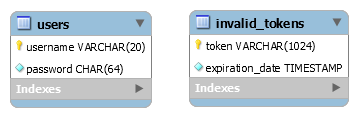
\includegraphics{AuthenticationER}
  \caption{Diagramma E/R del servizio \textit{Authentication Service}.}
\end{figure}

\section{Room Service}

\textit{Room Service} è il servizio che gestisce le \textit{chat room} di conversazione degli utenti. In particolare si occupa della creazione, eliminazione, adesione alle stanze e della persistenza dei messaggi.
Questo servizio è autonomo, non dipende da altri servizi.\\
Le risorse messe a disposizione dal servizio, specificate nella tabella \ref{tab:table_room}, permettono di:

\begin{itemize}
%
    \item \textbf{Creare} una stanza: l'utente fornisce il proprio \textit{username} e il \textit{nome} della stanza che vuole creare. Se l'operazione viene conclusa con successo il servizio risponde confermando la creazione \textit{Create} e inviando il \textit{nome} della stanza appena creata. Se l'operazione fallisce viene inviato un messaggio di errore \textit{Internal Server Error}. Se esiste già una stanza con quel nome, \textit{Room Service} risponde con messaggio di errore \textit{Conflict}.  Se \textit{username} e/o \textit{name} non sono presenti nella richiesta, il servizio restituisce il messaggio di errore \textit{Precondition Failed}.
%
    \item \textbf{Eliminare} una stanza: l'utente fornisce il proprio \textit{username} e il \textit{nome} della stanza come \textit{parametri} della richiesta. Il servizio controlla l'effettiva esistenza della stanza: se esiste il servizio conferma l'eliminazione con messaggio di accettazione \textit{OK}, altrimenti risponde con messaggio di errore \textit{Not Found}.  Se \textit{username} e/o \textit{name} non sono presenti nella richiesta, il servizio restituisce il messaggio di errore \textit{Precondition Failed}. Se l'operazione non viene conclusa correttamente il servizio risponde con \textit{Internal Server Error}.
%
    \item \textbf{Unirsi} ad una stanza: l'utente fornisce il proprio \textit{username} e il \textit{nome} della stanza come \textit{parametri} della richiesta. Se la stanza esiste, il servizio conferma la creazione della partecipazione dell'utente nella stanza \textit{Create}, altrimenti risponde con messaggio di errore \textit{Not Found}. Se \textit{username} e/o \textit{name} non sono presenti nella richiesta, il servizio restituisce il messaggio di errore \textit{Precondition Failed}. Se l'operazione non va a buon fine il servizio risponde con \textit{Internal Server Error}.
%
    \item \textbf{Abbandonare} una stanza: l'utente fornisce il proprio \textit{username} e il \textit{name} della stanza che vuole abbandonare. Se il token è valido, l'utente può disponnettersi e il servizio segna il token come non più utilizzabile, \textit{invalid}. Se i valori richiesti non sono presenti, il servizio risponde con un messaggio di errore \textit{Precondition Failed}. Se lo \textit{username} dell'utente o il \textit{name} della stanza non risultano presenti nel \textit{database}, il servizio restituisce il messaggio di errore \textit{Not Found}. Se l'operazione non viene conclusa correttamente il servizio risponde con \textit{Internal Server Error}.
%
    \item \textbf{Inviare} messaggi in una stanza: questa funzionalità permette la condivisione dei messaggi all'interno delle stanze. Infatti all'invio di un messaggio, viene creata una richiesta con \textit{username} dell'utente e \textit{content} del messaggio. Se l'operazione va a buon fine \textit{Create}, il \textit{RoomService} genera una risposta con il \textit{content} e il \textit{timestamp} del messaggio, il \textit{name} della stanza e lo \textit{username} dell'utente. Se i campi richiesti non sono presenti o non sono corretti, il servizio risponde rispettivamente con il messaggio di errore \textit{Precondition Failed}, oppure con messaggio di errore \textit{Not Found}. Se l'operazione non va a buon fine il servizio risponde con \textit{Internal Server Error}.
%
\end{itemize}

\begin{table}[H]
\centering
\resizebox{\columnwidth}{!}{%
\begin{tabular}{|l|l|c|c|c|l|}
\hline
\begin{tabular}[c]{@{}l@{}}HTTP\\ verb\end{tabular} & Resource                             & \begin{tabular}[c]{@{}c@{}}Request\\ Body\end{tabular}      & \begin{tabular}[c]{@{}c@{}}Response\\ Body\end{tabular}                      & Responses                                                    & \multicolumn{1}{c|}{Description}                                                                    \\ \hline
POST                                                & /rooms/                              & \begin{tabular}[c]{@{}c@{}}username, \\ name\end{tabular}   & name                                                                         & \begin{tabular}[c]{@{}c@{}}201, 412,\\ 500\end{tabular}      & Creazione stanza                                                                                    \\ \hline
GET                                                 & /rooms/                              & -                                                           & list of Room                                                                 & 200                                                          & Recupera la lista delle stanze                                                                      \\ \hline
DELETE                                              & /rooms/:name                         & username                                                    & name                                                                         & \begin{tabular}[c]{@{}c@{}}200, 404,\\ 412, 500\end{tabular} & Eliminazione stanza                                                                                 \\ \hline
POST                                                & /rooms/:name/participations          & username                                                    & participation                                                                & \begin{tabular}[c]{@{}c@{}}201, 404,\\ 412, 500\end{tabular} & Adesione alla stanza                                                                                \\ \hline
GET                                                 & /rooms/:name/participations          & -                                                           & list of Participations                                                       & 200                                                          & \begin{tabular}[c]{@{}l@{}}Recupera la lista delle\\ partecipazioni della stanza data\end{tabular}  \\ \hline
GET                                                 & /users/:username/participations      & -                                                           & list of Participations                                                       & 200                                                          & \begin{tabular}[c]{@{}l@{}}Recupera la lista delle\\ partecipazioni dell'utente dato\end{tabular}   \\ \hline
DELETE                                              & rooms/:name/participations/:username & -                                                           & name, username                                                               & \begin{tabular}[c]{@{}c@{}}200, 404,\\ 412, 500\end{tabular} & Abbandono della stanza                                                                              \\ \hline
POST                                                & rooms/:name/messages                 & \begin{tabular}[c]{@{}c@{}}content,\\ username\end{tabular} & \begin{tabular}[c]{@{}c@{}}content, timestamp,\\ username, name\end{tabular} & \begin{tabular}[c]{@{}c@{}}201, 404,\\ 412, 500\end{tabular} & Invio messaggio                                                                                     \\ \hline
GET                                                 & rooms/:name/messages                 & -                                                           & list of Messages                                                             & 200                                                          & \begin{tabular}[c]{@{}l@{}}Recupera la lista dei messaggi\\ presenti nella stanza data\end{tabular} \\ \hline
\end{tabular}
}
\captionof{table}{Risorse esposte dal \textit{Room Service}.} \label{tab:table_room} 
\end{table}

\begin{figure}[H]
  \centering
    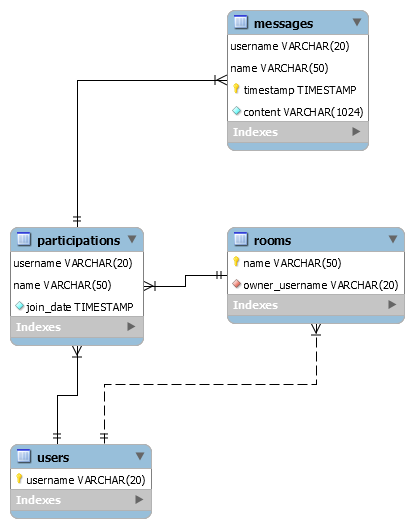
\includegraphics[scale=0.5]{RoomER}
  \caption{Diagramma E/R del servizio \textit{Room Service}.}
\end{figure}

\section{User Service}

\textit{User Service} è il servizio che gestisce il \textit{profilo} di ogni utente registrato all'applicazione. In particolare si occupa della creazione, eliminazione e aggiornamento dei profili utente.
Questo servizio è autonomo, non dipende da altri servizi.\\
Le risorse messe a disposizione dal servizio, specificate nella tabella \ref{tab:table_user}, permettono di:

\begin{itemize}
%
    \item \textbf{Creare} un utente: l'utente fornisce il proprio \textit{nome utente}, \textit{nome} e \textit{cognome}. Se l'operazione viene conclusa con successo il servizio risponde confermando la creazione con il messaggio \textit{Create} e inviando il \textit{profilo} dell'utente appena creato. Se l'operazione fallisce il servizio risponde con il messaggio di errore \textit{Internal Server Error}. Se esiste già un utente col \textit{nome utente} fornito in input il servizio risponde con il messaggio di errore \textit{Conflict}.  Se \textit{nome utente}, \textit{nome}, o \textit{cognome} non sono presenti nella richiesta il servizio risponde con il messaggio di errore \textit{Precondition Failed}.
%
    \item \textbf{Eliminare} un utente: l'utente fornisce il proprio \textit{nome utente}. Se l'operazione viene conclusa con successo il servizio risponde confermando l'eliminazione dell'utente con il messaggio \textit{(OK)} e inviando il \textit{nome utente} dell'utente appena eliminato. Se l'operazione fallisce il servizio risponde con il messaggio di errore \textit{Internal Server Error}. Se non esiste un utente con il \textit{nome utente} specificato il servizio risponde con il messaggio di errore \textit{Not Found}. Se il \textit{nome utente} non è presente nella richiesta il servizio risponde con il messaggio di errore \textit{Precondition Failed}.
%
    \item \textbf{Aggiornare} il profilo utente: l'utente fornisce il proprio \textit{nome utente} oltre al nuovo \textit{nome}, \textit{cognome} e \textit{biografia}. Se l'operazione viene conclusa con successo il servizio risponde confermando l'aggiornamento del profilo utente rispondendo con il messaggio \textit{OK} e inviando il \textit{profilo} aggiornato dell'utente che ha effettuato la richiesta. Se l'operazione fallisce il servizio risponde con il messaggio di errore \textit{Internal Server Error}. Se non esiste un utente con il \textit{nome utente} specificato il servizio risponde con il messaggio di errore \textit{Not Found}. Se \textit{nome utente}, \textit{nome}, \textit{cognome} o \textit{biografia} non sono presenti nella richiesta il servizio risponde con il messaggio di errore \textit{Precondition Failed}.
%
    \item \textbf{Recuperare} il profilo utente: l'utente fornisce il proprio \textit{nome utente}. Se l'operazione viene conclusa con successo il servizio risponde confermando l'aggiornamento del profilo utente rispondendo con il messaggio \textit{OK} e inviando il profilo dell'utente che ha effettuato  la richiesta. Se l'operazione fallisce il servizio risponde con il messaggio di errore \textit{Internal Server Error}. Se non esiste un utente con il \textit{nome utente} specificato il servizio risponde con il messaggio di errore \textit{Not Found}. Se \textit{nome utente} non \`e presente nella richiesta il servizio risponde con il messaggio di errore \textit{Precondition Failed}.
%
\end{itemize}

\begin{table}[H]
\centering
\resizebox{\columnwidth}{!}{%
\begin{tabular}{|l|l|c|c|c|c|l|}
\hline
\begin{tabular}[c]{@{}l@{}}HTTP\\ verb\end{tabular} & Resource                              & \multicolumn{1}{l|}{Header} & \begin{tabular}[c]{@{}c@{}}Request\\ Body\end{tabular}                                  & \begin{tabular}[c]{@{}c@{}}Response\\ Body\end{tabular}   & Responses                                                     & \multicolumn{1}{c|}{Description}          \\ \hline
POST                                                & /users                                & -                           & \begin{tabular}[c]{@{}c@{}}username, \\ firstName, \\ lastName\end{tabular}             & User profile                                              & \begin{tabular}[c]{@{}c@{}}201, 409, 412,\\ 500\end{tabular}  & Creazione di un utente                    \\ \hline
GET                                                 & /users/:username                      & -                           & -                                                                                       & User profile                                              & \begin{tabular}[c]{@{}c@{}}200, 404,\\ 412, 500\end{tabular}  & Recuperare il profilo di un utente        \\ \hline
PUT                                                 & /users/:username                      & -                           & \begin{tabular}[c]{@{}c@{}}firstName, \\ lastName, \\ bio, \\ visible \end{tabular}     & User profile                                              & \begin{tabular}[c]{@{}c@{}}200, 404,\\ 412, 500\end{tabular}  & Aggiornamento del profilo di un utente    \\ \hline
DELETE                                              & /users/:username                      & -                           & -                                                                                       & username                                                  & \begin{tabular}[c]{@{}c@{}}200, 404,\\ 412, 500\end{tabular}  & Eliminazione di un utente                 \\ \hline
PUT                                                 & /users/:username/access               & -                           & -                                                                                       & -                                                         & \begin{tabular}[c]{@{}c@{}}200, 500\end{tabular}  & Aggiornamento ultimo accesso              \\ \hline
\end{tabular}
}
\captionof{table}{Risorse esposte dallo \textit{User Service}.} \label{tab:table_user} 
\end{table}

\begin{figure}[H]
  \centering
    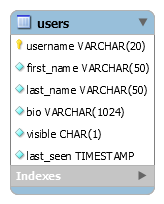
\includegraphics{UserER}
  \caption{Diagramma E/R del servizio \textit{User Service}.}
\end{figure}

\section{Web App Service}

\textit{Web App Service} è il servizio che si occupa di inoltrare le richieste effettuate dai client ai relativi servizi, di gestire la parte di aggiornamento in tempo reale dei singoli client (per es. propaganzione di un messaggio a tutti gli utenti attivi presenti all'interno di una stanza) e di servire l'applicazione web all'utente.

Per erogare tutte le funzionalit\`a esposte il \textit{Web App Service} si appoggia sui servizi di back-end descritti in precedenza. Per esempio per registrare un utente si appoggia sull'\textit{Authentication Service} per archiviare le credenziali di autenticazione e sullo \textit{User Service} per archiviare il profilo utente.

Le risorse messe a disposizione dal servizio sono specificate nella tabella \ref{tab:table_webapp}.

\begin{table}[H]
\centering
\resizebox{\columnwidth}{!}{%
\begin{tabular}{|l|l|c|c|c|c|l|}
\hline
\begin{tabular}[c]{@{}l@{}}HTTP\\ verb\end{tabular} & Resource                             & Header & \begin{tabular}[c]{@{}c@{}}Request\\ Body\end{tabular}                                & \begin{tabular}[c]{@{}c@{}}Response\\ Body\end{tabular} & Responses                                                           & \multicolumn{1}{c|}{Description}                                                                       \\ \hline
POST                                                & /register                            & -      & \begin{tabular}[c]{@{}c@{}}username, \\ firtname,\\ lastname,\\ password\end{tabular} & User                                                    & \begin{tabular}[c]{@{}c@{}}201, 412,\\ 500\end{tabular}             & Creazione utente                                                                                       \\ \hline
POST                                                & /login                               & -      & \begin{tabular}[c]{@{}c@{}}username,\\ password\end{tabular}                          & User                                                    & \begin{tabular}[c]{@{}c@{}}200, 404,\\ 412\end{tabular}             & Login utente                                                                                           \\ \hline
DELETE                                              & /logout                              & token  & username                                                                              & -                                                       & \begin{tabular}[c]{@{}c@{}}204, 401, 404,\\ 412, 500\end{tabular}   & Logout utente                                                                                          \\ \hline
GET                                                 & /rooms                               & token  & -                                                                                     & list of Rooms                                           & \begin{tabular}[c]{@{}c@{}}200, 401,\\ 404,\\ 412, 500\end{tabular} & \begin{tabular}[c]{@{}l@{}}Recupera la lista delle stanze\\ in cui l'utente non partecipa\end{tabular} \\ \hline
POST                                                & /rooms                               & token  & \begin{tabular}[c]{@{}c@{}}usernane,\\ name\end{tabular}                              & name                                                    & \begin{tabular}[c]{@{}c@{}}200, 401,\\ 404,\\ 412, 500\end{tabular} & Creazione stanza                                                                                       \\ \hline
DELETE                                              & /rooms/:name                         & token  & username                                                                              & -                                                       & \begin{tabular}[c]{@{}c@{}}204 401,\\ 404,\\ 412, 500\end{tabular}  & Eliminazione stanza                                                                                    \\ \hline
POST                                                & /rooms/:name/participations          & token  & username                                                                              & Participation                                           & \begin{tabular}[c]{@{}c@{}}201, 401,\\ 404,\\ 412, 500\end{tabular} & Adesione alla stanza                                                                                   \\ \hline
GET                                                 & /rooms/:name/participations          & token  & -                                                                                     & list of Participations                                  & \begin{tabular}[c]{@{}c@{}}200, 401,\\ 404,\\ 412, 500\end{tabular} & \begin{tabular}[c]{@{}l@{}}Recupera la lista delle\\ partecipazioni della stanza data\end{tabular}     \\ \hline
DELETE                                              & rooms/:name/participations/:username & token  & -                                                                                     & name, username                                          & \begin{tabular}[c]{@{}c@{}}200, 404,\\ 412, 500\end{tabular}        & Abbandono della stanza                                                                                 \\ \hline
POST                                                & rooms/:name/messages                 & token  & \begin{tabular}[c]{@{}c@{}}content,\\ username\end{tabular}                           & Message                                                 & \begin{tabular}[c]{@{}c@{}}201, 404,\\ 412, 500\end{tabular}        & Invio messaggio                                                                                        \\ \hline
GET                                                 & rooms/:name/messages                 & token  & -                                                                                     & list of Messages                                        & \begin{tabular}[c]{@{}c@{}}200, 401,\\ 404,\\ 412, 500\end{tabular} & \begin{tabular}[c]{@{}l@{}}Recupera la lista dei messaggi\\ presenti nella stanza data\end{tabular}    \\ \hline
GET                                                 & /users/:username                     & token  & -                                                                                     & User                                                    & \begin{tabular}[c]{@{}c@{}}200, 404,\\ 412, 500\end{tabular}        & \begin{tabular}[c]{@{}l@{}}Recupera l'utente dato\\ il suo username\end{tabular}                       \\ \hline
PUT                                                 & /users/:username                     & token  & \begin{tabular}[c]{@{}c@{}}firtname,\\ lastname,\\ bio,\\ visible\end{tabular}        & User                                                    & \begin{tabular}[c]{@{}c@{}}200, 404,\\ 412, 500\end{tabular}        & Update utente                                                                                          \\ \hline
DELETE                                              & /users/:username                     & token  & -                                                                                     & username                                                & \begin{tabular}[c]{@{}c@{}}204, 401,\\ 404,\\ 412, 500\end{tabular} & Eliminazione utente                                                                                    \\ \hline
GET                                                 & /users/:username/participations      & token  & -                                                                                     & list of Participations                                  & \begin{tabular}[c]{@{}c@{}}200, 401,\\ 404,\\ 412, 500\end{tabular} & \begin{tabular}[c]{@{}l@{}}Recupera la lista delle\\ partecipazioni di un\\ dato utente\end{tabular}   \\ \hline
\end{tabular}
}
\captionof{table}{Risorse esposte dallo \textit{User Service}.} \label{tab:table_webapp} 
\end{table}

\section{Client}
Il front-end del sistema è un'Applicazione Web realizzata in Angular e servita dal \texttt{WebAppService}.
L'applicazione si presenta con una prima pagina di \textit{login}, dove l'utente potrà inserire il suo \textit{username} e la \textit{password}. Nel caso l'utente non fosse ancora registrato, ha a possibilità di registrarsi e creare un proprio profilo.

Una volta effettuato l'accesso la pagina presenta:
\begin{enumerate*}[label=(\arabic*)]
    \item un menù laterale in cui sono visibili le stanze a cui l'utente ha ito,
    \item una funzionalità di \textit{ricerca} delle stanze,
    \item una funzionalità che permette la \textit{creazione} di nuove stanze,
    \item un bottone per il logout e la modifica del profilo utente,
    \item la chat di messaggistica che mostra i messaggi scambiati dagli utenti,
    \item un bottone che permette di vedere le informazioni riguardanti una stanza, in particolare i partecipanti alla chat e il loro profilo.
\end{enumerate*}


\chapter{Implementazione}

In questo capitolo sono analizzati nel dettaglio i contributi apportati da ciascun componente del gruppo.

Avendo impostato il sistema basandoci sulla \textit{Clean Architecture}, in cui la modellazione delle funzionalità del sistema viene trattata in termini di casi d'uso (\textit{interattori}), gran parte del carico di lavoro è stato suddiviso tra i membri del team attraverso la  \textbf{spartizione dei casi d'uso} da implementare.
Per la creazione dei micro-servizi sono state utilizzate le librerie messe a disposizione da Vert.x. 

\section{Componenti creati in cooperazione}

Bootstrapping dell'Architettura:

\begin{itemize}
    \item Identificazione e design dei servizi richiesti
    \item Identificazione delle sorgenti necessari per ogni servizio e design dei \textit{DB}
    \item Identificazione e preparazione della piattaforma DBaaS 
    \item Creazione degli Use Case Diagram in UML
    \item Creazione dei Class Diagram in UML
    \item Creazione dei Sequence Diagram in UML
\end{itemize}

\section{Alessandro}
Lo studente \textit{Alessandro Gnucci} si è occupato dello sviluppo dei seguenti items, definiti nel \textit{Product Backlog}:
\begin{itemize}
    \item \textbf{Architecture bootstrapping} (con il resto del team). Questa parte si articola in:
    \begin{itemize}
        \item Identificazione dei servizi richiesti;
        \item Identificazione delle sorgenti dati per i servizi e design dei \textit{DB};
        \item Identificazione e preparazione della piattaforma \textit{DBaaS}, inoltre design dell'\textit{UML Use Case Diagram}.
        \item  Design dell'\textit{UML Class Diagram}.
    \end{itemize}
    
    \item \textbf{Registrazione di un utente}
        \begin{itemize}
            \item Design del diagramma \textit{UML} di sequenza (con il resto del team).
            \item Implementazione \textit{TDD} del \textit{Authentication Service}.
        \end{itemize}
    
    \item \textbf{Login di un utente}
        \begin{itemize}
            \item Design del diagramma \textit{UML} di sequenza (con il resto del team).
            \item Implementazione \textit{TDD} dell'\textit{Authentication Service}.
        \end{itemize}
        
    \item \textbf{Logout}
    \begin{itemize}
        \item Design del diagramma \textit{UML} di sequenza (con il resto del team).
        \item Implementazione \textit{TDD} dell'\textit{Authentication Service}.
    \end{itemize}
    
    \item \textbf{Controllo di validità dei tokens Jwt}: 
    implementazione \textit{TDD} dell'\textit{Authentication Service}.
        
     \item \textbf{Rimozione di una stanza}: 
    \begin{itemize}
        \item implementazione \textit{TDD} del \textit{WebApp Service}.
        \item implementazione \textit{TDD} del \textit{Room Service}.
        \item Implementazione \textit{TDD} del \textit{Web Client}.
    \end{itemize}   
        
    \item \textbf{Ricerca di una stanza}: implementazione \textit{TDD} del \textit{Room Service}.

    \item \textbf{Cancellazione di un account}: implementazione \textit{TDD} 
    dell'\textit{Authentication Service}.
        
    \item \textbf{Refactoring del codice dei servizi}: refactoring del codice 
    dell'\textit{Authentication Service}.
    
    \item \textbf{Abbandono da parte di un utente di una stanza}: 
    \begin{itemize}
        \item implementazione \textit{TDD} del \textit{WebApp Service}.
        \item implementazione \textit{TDD} del \textit{Room Service}.
        \item Implementazione \textit{TDD} del \textit{Web Client}.
    \end{itemize}  
    
    \item \textbf{Modifica del profilo utente}: 
    \begin{itemize}
        \item implementazione \textit{TDD} del \textit{WebApp Service}.
        \item implementazione \textit{TDD} del \textit{User Service}.
        \item Implementazione \textit{TDD} del \textit{Web Client}.
    \end{itemize}  
    
    \item \textbf{Aggiornamento in real-time sullo stato di scrittura degli utenti nelle stanze}: 
    \begin{itemize}
        \item implementazione \textit{TDD} del \textit{WebApp Service}.
        \item Implementazione \textit{TDD} del \textit{Web Client}.
    \end{itemize}  
    
\end{itemize}

\section{Nicola}
All'interno del progetto \textit{Distributed Chat Service}, lo studente \textit{Nicola Piscaglia} si è occupato dello sviluppo dei seguenti item definiti nel \textit{Product Backlog}:
\begin{itemize}
    \item \textbf{Project bootstrapping}: in particolare dell'inizializzazione e configurazione di \textit{Travis CI}.
    
    \item \textbf{Architecture bootstrapping} (in cooperazione con gli altri membri del team). In particolare questa fase si è articolata in:
    \begin{itemize}
        \item Identificazione dei servizi richiesti (si è scelto di utilizzare l'architettura a microservizi).
        \item Identificazione delle sorgenti dati necessarie per ogni servizio e design del \textit{DB}.
        \item Identificazione/creazione della piattaforma \textit{DBaaS} e design dell'\textit{UML Use Case Diagram}.
        \item \textit{UML Class Diagram} Design.
    \end{itemize}
    
    \item \textbf{Registrazione di un utente}
        \begin{itemize}
            \item Design del diagramma \textit{UML} di sequenza (in cooperazione con gli altri membri del team).
            \item Implementazione \textit{TDD} del \textit{WebApp Service}.
        \end{itemize}
    
    \item \textbf{Login}
        \begin{itemize}
            \item design del diagramma \textit{UML} di sequenza (in cooperazione con gli altri membri del team).
            \item Implementazione \textit{TDD} del \textit{WebApp Service}.
        \end{itemize}
    
    \item \textbf{Logout}
        \begin{itemize}
            \item Design del diagramma \textit{UML} di sequenza (in cooperazione con gli altri membri del team).
            \item Implementazione \textit{TDD} del \textit{WebApp Service}.
        \end{itemize}
        
     \item \textbf{Creazione di una stanza}: implementazione \textit{TDD} del \textit{WebApp Service}.
     
     \item \textbf{Rimozione di una stanza}: implementazione del \textit{Web Client}.
    
    \item \textbf{Validazione dell'input}: implementazione della validazione delle richieste di ogni servizio.
    
    \item \textbf{Partecipazione ad una stanza}:
        \begin{itemize}
            \item implementazione del \textit{Web Client}.
            \item implementazione \textit{TDD} del \textit{WebApp Service}.
        \end{itemize}
        
    \item \textbf{Refactoring del codice dei servizi}: refactoring del codice del \textit{WebApp Service}.
    
    \item \textbf{Standardizzazione delle Rest API}: in particolare sono state uniformate le chiamate REST e le rotte in base al design formalizzato tramite specifica \textit{Swagger}. Tali cambiamenti hanno impattato i seguenti componenti:
        \begin{itemize}
            \item \textit{WebApp Service}
            \item \textit{Room Service}
            \item \textit{User Service}
            \item \textit{Authentication Service}
            \item \textit{Web Client}
        \end{itemize}
    
    \item \textbf{Visualizzazione delle informazioni di una stanza}
    \begin{itemize}
        \item Implementazione \textit{TDD} del \textit{WebApp Service}.
        \item Implementazione \textit{TDD} del \textit{Room Service}.
        \item Implementazione del \textit{Web Client}.
    \end{itemize}
    
    \item \textbf{Visualizzazione del profilo di altri utenti}
    \begin{itemize}
        \item Implementazione \textit{TDD} del \textit{WebApp Service}.
        \item Implementazione \textit{TDD} dello \textit{User Service}.
        \item Implementazione del \textit{Web Client}.
    \end{itemize}
    
\end{itemize}


\section{Martina}

All'interno del progetto \textit{Distributed Chat Service} la studentessa \textit{Magnani Martina} si è occupata dello sviluppo delle seguenti parti:

\begin{itemize}
    \item Registrazione di un utente:
    \begin{itemize}
        \item Implementazione TDD del micro-servizio \textit{User Service}.
    \end{itemize}
    \item Login di un utente:
    \begin{itemize}
        \item Implementazione TDD del micro-servizio \textit{User Service}.
    \end{itemize}
    \item Creazione di una stanza:
    \begin{itemize}
        \item Implementazione TDD del micro-servizio \textit{Room Service}.
        \item Implementazione del \textit{Web Client} in cooperazione con \textit{Vandi Mattia}.
        \item Debug e testing (Sevice \& Web Client) della funzionalità ai fini della \textit{release}.
    \end{itemize}
    \item Refactoring del codice dei servizi:
    \begin{itemize}
        \item Refactoring del codice del micro-servizio \textit{User Service}.
    \end{itemize}
    \item Ricerca di una stanza:
    \begin{itemize}
        \item Implementazione TDD del micro-servizio \textit{WebApp Service}.
    \end{itemize}
    \item Partecipazione ad una stanza:
    \begin{itemize}
        \item Implementazione TDD del micro-servizio \textit{Room Service}.
    \end{itemize}
    \item Invio di un messaggio:
    \begin{itemize}
        \item Implementazione TDD del micro-servizio \textit{Room Service}.
        \item Implementazione TDD del micro-servizio \textit{WebApp Service}.
        \item Implementazione del \textit{Web Client}.
    \end{itemize}
    \item Ricezione di un messaggio:
    \begin{itemize}
        \item Implementazione TDD del micro-servizio \textit{Room Service}.
        \item Implementazione TDD del micro-servizio \textit{WebApp Service}.
        \item Implementazione del \textit{Web Client}.
    \end{itemize}
    \item Ricezione dei messaggi passati per le stanze in cui l'utente partecipa:
    \begin{itemize}
        \item Implementazione TDD del micro-servizio \textit{Room Service}.
        \item Implementazione TDD del micro-servizio \textit{WebApp Service}.
        \item Implementazione del \textit{Web Client}.
    \end{itemize}
\end{itemize}

\section{Mattia}

All'interno del progetto \textit{Distributed Chat Service} lo studente \textit{Vandi Mattia} si è occupato dello sviluppo delle seguenti parti:

\begin{itemize}
%
    \item Bootstrapping del progetto:
%
    \begin{itemize}
%
        \item Inizializzazione del repository.
%
        \item Inizializzazione della configurazione multi-progetto Gradle.
%
        \item Inizializzazione di Trello.
%
    \end{itemize}
%
    \item Registrazione di un utente:
%
    \begin{itemize}
%
        \item Implementazione TDD nel micro-servizio \textit{User Service}.
%
        \item Implementazione del \textit{Web Client}.
%
    \end{itemize}
%
    \item Creazione di una stanza:
%
    \begin{itemize}
%
        \item Implementazione del \textit{Web Client}.
%
    \end{itemize}
%
    \item Eliminazione di una stanza:
%
    \begin{itemize}
%
        \item Implementazione TDD nel micro-servizio \textit{Room Service}.
%
    \end{itemize}
%
    \item Ricerca di una stanza:
%
    \begin{itemize}
%
        \item Implementazione del \textit{Web Client}.
%
    \end{itemize}
%
    \item Refactoring del micro-servizio \textit{Room Service}.
%
    \item Broadcasting degli eventi di creazione e eliminazione di una stanza.
%
    \begin{itemize}
%
        \item Implementazione TDD nel micro-servizio \textit{Web App Service}.
%
        \item Implementazione del \textit{Web Client}.
%
    \end{itemize}
%
    \item Definizione di una descrizione formale dei micro-servizi utilizzando il tool Swagger.
%
    \item Invisibilità dell'utente:
%
    \begin{itemize}
%
        \item Implementazione TDD nel micro-servizio \textit{Room Service}.
%
        \item Implementazione TDD nel micro-servizio \textit{Web App Service}.
%
        \item Implementazione del \textit{Web Client}.
%
    \end{itemize}
%
\end{itemize}

\chapter{Retrospettiva}

\section{Processo di sviluppo}

Il lavoro è stato organizzato secondo le filosofie della metodologia Agile, adottando un approccio \textit{Scrum-like}.
%
Non dispondendo della figura dello scrum manager il team si è autorganizzato e autogestito per la definizione dei task da portare a termine negli Sprint settimanai e per la loro distrubuzione tra i membri.

Al termine di ogni Sprint i componenti hanno preso parte a un meeting, durante il quale sono state poste in atto le fasi di \textit{Sprint Review} (per valutare il risultato dello Sprint e stabilire le priorità delle prossime feature da portare a termine) e di \textit{Sprint Retrospective} (per analizzare il processo di sviluppo allo scopo di migliorare la produttività del team).

Il codice è stato sviluppato usando tecniche di \textit{Test-Driven-Development} (TDD).

Per aiutarci nella pianificazione degli Sprint settimanali abbiamo utilizzato \textit{Google Sheets} per tenere traccia sia del product backlog complessivo sia del product backlog degli Sprint settimanali.
%
Abbiamo utilizzato \textit{Trello} per tracciare l'andamento dei task asseganti.

\section{Andamento degli Sprint}

\subsection{Sprint 1}

Le funzionalità che ci siamo prefissi di sviluppare all'interno di questo Sprint sono:

\begin{itemize}
%
    \item Possibilità di registrazione di un nuovo utente.
%
    \item Possibilità di effettuare l'accesso da parte di un utente già presente all'interno del sistema.
%
    \item Possibilità, da parte di un utente che ha già effettuato l'accesso, di uscire dall'applicazione.
%
\end{itemize}

Nella fase iniziale dello \textit{Sprint} ci siamo concentrati sul bootstrapping del progetto, in particolare è stato inizializzato il repository e gli strumenti di supporto alla \textit{continuous integration} (Travis CI, Gradle, Trello e Google Sheets).

Successivamente siamo passati ad una fase di analisi e modellazione del problema, in particolare abbiamo identificato l'architettura del sistema e definito lo schema delle \textit{basi di dati}.
%
Sono stati prodotti i diagrammi UML di massima del dominio applicativo (casi d'uso e diagramma delle classi).

In seguito, abbiamo modellato ciascun caso d'uso di competenza dello Sprint con dei diagrammi di sequenza e l'architettura di ogni microservizio con diagrammi delle classi. Questa parte ha richiesto più tempo del previsto e ha sottratto diverso tempo alla fase successiva di implementazione di ogni servizio.
%
Quest'ultima fase è stata iniziata ma non terminata all'interno di questo Sprint.

\subsubsection{Retrospettiva}

Analizzando il processo di sviluppo adottato in questo Sprint è emerso che alcuni task sono stati sottostimati.
%
In particolare, abbiamo attribuito una grandezza inferiore alle fasi di modellazione e sviluppo, di conseguenza negli Sprint successivi verranno calibrati meglio i task per ogni sprint. In particolare task troppo onerosi saranno scomposti in sotto-task più piccoli da distribuire in più sprint.

\subsection{Sprint 2}

In questo Sprint è stata terminata l'implementazione lato \textit{server} delle funzionalità che non erano state completate nello Sprint precedente ed è stato applicato in maniera sistematica lo \textit{unit-testing} durante la fase di sviluppo.

Inoltre è stata iniziata l'implementazione del client in \textit{Angular}: architettura generale, componenti principali e impostazione del \textit{template}.

\subsubsection{Retrospettiva}

I risultati di questo Sprint sono stati abbastanza soddisfacenti, in quanto è stato applicato il processo di TDD per tutti i test delle Web API di ogni servizio.

A livello di processo di processo di sviluppo, negli Sprint successivi, saranno effettuate \textit{pull request} più frequenti al fine di risolvere un minor numero di conflitti durante la fusione delle singole \textit{pull request}.

\subsection{Sprint 3}

In questo Sprint sono state aggiunte le seguenti funzionalità:

\begin{itemize}
%
    \item Aggiunta di una nuova stanza.
%
    \item Eliminazione di una stanza.
%
    \item Controllo della validità del token passato da un utente.
%
\end{itemize}

In questo Sprint ogni membro del team ha terminato i task assegnati. È stata ultimata l'implementazione dei microservizi in merito ai casi d'uso che erano stati prefissati.

\subsubsection{Retrospettiva}

Gli elementi assegnati a questa settimana si sono dimostrati correttamente quantificati per questo abbiamo ritenuto che l'aggiunta di ulteriori task per i successivi Sprint non sia necessaria.
Tutti i membri sono riusciti a completare i propri compiti nell'arco della settimana.

Per lo Sprint successivo ci cercherò di portare a termine lo sviluppo di un prototipo funzionante in base ai casi d'uso implementati finora.

\subsection{Sprint 4}

In questo Sprint ci siamo dedicati al \textit{debug} delle funzionalità sviluppate fino a questo momento, sia lato client sia lato servizi.

Abbiamo cambiato il \textit{layout} dell'applicazione web applicando un nuovo \textit{template} che consente una prototipazione più facile dell'interfaccia utente.

Abbiamo introdotto la validazione delle richieste effettuate dall'utente in ogni servizio.

Ė stato uno Sprint particolarmente impegnativo dal punto di vista del carico di lavoro; in particolare per la validazione dell'input delle richieste di ogni servizio. Siamo comunque riusciti a completare con successo tutti i tasks prefissati.
È stato raggiunto l'obiettivo di realizzare un prototipo funzionante che implementasse i casi d'uso finora delineati.

\subsubsection{Retrospettiva}

I tasks assegnati sono stati completati anche se non è rimasto tempo per ulteriori migliorie o refactoring del codice. Nel prossimo Sprint vogliamo riservare spazio anche per aumentare il numero di test e riportare la qualità del codice ad un livello più alto.

\subsection{Sprint 5}

In questo Sprint sono state aggiunte le seguenti funzionalità:

\begin{itemize}
%
    \item Ricerca di una stanza da parte di un utente.
%
    \item Possibilità, da parte di un utente, di unirsi ad una stanza già esistente.
%
\end{itemize}

\`E stato aggiunto il broadcasting dell'evento di creazione di una stanza, in modo tale che ogni client possa essere informato, durante la fase di ricerca di una stanza quando una nuova stanza è stata aggiunta senza aver bisogno di effettuare una nuova ricerca.

I task per questo Sprint sono stati completati con successo, a meno della ricerca delle stanze. In particolare è incompleta la parte client.
\`E stata definita, inoltre, una specifica standard per le rotte dei servizi \textit{REST}, tramite \textit{Swagger}. Quindi nel prossimo Sprint, si dovranno adattare le rotte già implementate alla specifica delineata.

\subsubsection{Retrospettiva}

In questo Sprint è stato aggiornato il backlog con nuovi task in modo incrementale; l'obiettivo per lo Sprint successivo sarà quello di terminare i task prefissati al suo inizio, senza aggiungerne di nuovi nel corso dello Sprint.
Complessivamente, lo Sprint si è concluso senza particolari problemi.

\subsection{Sprint 6}

In questo Sprint sono state aggiunte le seguenti funzionalità:

\begin{itemize}
%
    \item Invio di un messaggio da parte di un utente.
%
    \item Ricezione di un messaggio da parte dell'utente.
%
    \item Possibilità da parte di utente di abbandonare una stanza.
%
    \item Possibilità da parte di utente di visualizzare le informazioni relative ad una stanza stanza.
%
\end{itemize}

\`E stata ultimata la standardizzazione delle interfacce \textit{REST} di ogni servizio ed è stata completata la ricerca delle stanze da parte dell'utente.

È stato uno Sprint a carattere decisamente implementativo, durante il quale sono state sviluppate diverse feature fondamentali per la web application (e.g. invio/ricezione di un messaggio, ricerca di una stanza, visualizzazione dei dettagli di una stanza, ecc.).
I compiti assegnati sono stati interamente completati.

\subsubsection{Retrospettiva}

Riteniamo che il team abbia previsto un carico di lavoro adeguato alle ore a disposizione. Lo sviluppo è stato particolarmente produttivo, grazie anche al maggior tempo a disposizione per l'implementazione di nuove feature.
Non è stato riscontrato nessun problema particoalare. La sfida dei prossimi Sprint, a livello di processo, sarà definire un piano di lavoro che porti alla terminazione dell'implementazione del sistema e alla scrittura della relazione di progetto, in tempo utile per la consegna finale.

\subsection{Sprint 7}

In questo Sprint sono state aggiunte le seguenti funzionalità:

\begin{itemize}
%
    \item Possibilità da parte di un utente di rendersi invisibile agli altri utenti.
%
    \item Possibilità di visualizzare il profilo degli altri utenti presenti in una chat.
%
    \item Possibilità di visualizzare in tempo reale l'aggioranmento sullo stato di scrittura da parte di utente.
%
    \item Possibilità di recuperare i messaggi precedentemente scambiati all'interno di una stanza.
%
\end{itemize}

In questo Sprint sono state sviluppate con successo tutte le funzionalità rimaste, escluse le opzionali, ottenendo così come risultato il sistema completo.

\subsubsection{Retrospettiva}

I tasks assegnati per questo Sprint si sono dimostrati correttamente quantificati. L'obbiettivo per lo Sprint successivo sarà quello di scrivere la relazione in maniera dettagliata, completa ed esaustiva.

\subsection{Sprint 8}

In questo Sprint il team si è dedicato alla stesura della Relazione di progetto.
È stato deciso di dividere il team in gruppi di due persone, in modo tale che alla fine del lavoro ogni gruppo ha potuto revisionare la parte dell'altro.
La relazione secondo le regole d'esame doveva essere formata da 6 capitoli; formando due gruppi, ognuno ha potuto scrivere esattamente 3 capitoli della relazione.

\subsubsection{Retrospective}

La divisione del lavoro è risultata corretta ai fini del completamento dello Sprint e della Relazione. Ci siamo resi conto che alcuni diagrammi UML realizzati in precedenza dovevano essere ampliati, in quanto definiti durante il primo Sprint e di conseguenza non coprivano ancora tutte le funzionalità che il sistema avrebbe implementato. 

\section{Commenti finali}
Avendo impostato il progetto seguendo la filosofia della \textit{Clean Architecture}, basata su una modellazione delle funzionalità in termini di casi d'uso (\textit{interattori}), il nostro codice risulta molto pulito, leggibile, riutilizzabile e facilmente manutenibile.

L'utilizzo delle \textit{pull request} messe a disposizione da \textit{GitHub} è risultato molto efficace durante lo sviluppo, in quanto ciascun membro del team ha potuto lavorare autonomamente nel proprio repository.
I vantaggi derivanti sono stati:
\begin{enumerate*}[label=(\arabic*)]
%
    \item un minor numero di conflitti durante lo sviluppo concorrente,
%
    \item il testing automatico di ciascuna feature prima di essere caricata (\textit{Continuous Integration} di \textit{TravisCI}) e
%
    \item autonomia nello sviluppo.
%
\end{enumerate*}

Anche l'approccio Agile è risultato molto comodo, ci ha permesso di organizzare al meglio i task da svolgere e l'obiettivo di soddisfare gli Sprint ha motivato tutto il gruppo a lavorare regolarmente e costantemente.
\`E stato riscontrato qualche problema solo durante le prime settimane, in quanto dovevamo capire il giusto peso da attribuire ai vari task e imparare il corretto approccio a questa metodologia di sviluppo, a noi nuova.

Ogni settimana, a partire dalla quarta, è stato rilasciato un prototipo di progetto che è stato arricchito di nuove funzionalità in maniera incrementale.
%
Durante i  primi Sprint ci siamo concentrati nella creazione della struttura base di tutti i servizi e del client. Successivamente abbiamo proceduto all'implementazione di tutti i casi d'uso seguendo una scaletta in ordine d'importanza decrescente.

Al termine del progetto il team si ritiene soddisfatto del lavoro svolto; tutti i requisiti funzionali sono stati completati ed è possibile utilizzare \textit{Distributed Chat Service} in maniera distribuita con aggiornamenti in tempo reale.
I servizi possono trovarsi su macchine differenti senza causare alcun problema all'esecuzione della chat.

\section{Estensioni future}

Pensando ad un prossimo sviluppo, ci piacerebbe estendere \textit{Distributed Chat Service} con le seguenti funzionalità:

\begin{itemize}
%
    \item Trasferimeto di file multimediali nelle chat.
%
    \item Suoni personalizzati all'arrivo dei messaggi a seconda del mittente e della stanza.
%
    \item Invio di note vocali.
%
    \item Integrazione di emoji.
%
    \item \textit{Chatbot} helper e di compagnia.
\end{itemize}



\end{document}
